\documentclass[11pt]{article}
\usepackage[T1]{fontenc}
\usepackage{lmodern}
\usepackage[margin=1.05in]{geometry}
\usepackage{amsmath,amssymb,amsthm,mathtools}
\usepackage{microtype}
\usepackage{enumitem}
\usepackage{booktabs}
\usepackage{xcolor}
\usepackage{tikz}
\usetikzlibrary{arrows.meta,positioning}
\usepackage{hyperref}
\hypersetup{colorlinks=true,linkcolor=blue!45!black,citecolor=blue!45!black,urlcolor=blue!45!black,pdftitle={Tensor saturation for even spin groups},pdfauthor={OpenAI}}
\newcommand{\R}{\mathbb R}
\newcommand{\C}{\mathbb C}
\newcommand{\Z}{\mathbb Z}
\newcommand{\N}{\mathbb N}
\newcommand{\Q}{\mathbb Q}
\newcommand{\eps}{\varepsilon}
\newcommand{\dd}{\,\mathrm d}
\DeclareMathOperator{\Spin}{Spin}
\DeclareMathOperator{\SO}{SO}
\DeclareMathOperator{\GL}{GL}
\DeclareMathOperator{\Sp}{Sp}
\DeclareMathOperator{\Hom}{Hom}
\DeclareMathOperator{\End}{End}
\DeclareMathOperator{\tr}{tr}
\DeclareMathOperator{\im}{im}
\DeclareMathOperator{\rk}{rk}
\DeclareMathOperator{\Ad}{Ad}
\newtheorem{theorem}{Theorem}[section]
\newtheorem{proposition}[theorem]{Proposition}
\newtheorem{lemma}[theorem]{Lemma}
\newtheorem{corollary}[theorem]{Corollary}
\theoremstyle{definition}
\newtheorem{definition}[theorem]{Definition}
\theoremstyle{remark}
\newtheorem{remark}[theorem]{Remark}
\newtheorem{example}[theorem]{Example}
\numberwithin{equation}{section}
\setlist{itemsep=2pt,topsep=5pt}
\setlength{\emergencystretch}{1em}
\title{Tensor saturation for even spin groups}
\author{OpenAI}
\date{September 24, 2026}
\begin{document}
\maketitle
\begin{abstract}
We prove the saturation conjecture for $\Spin(2n)$, $n\ge2$.
If three dominant integral weights sum to an element of the root lattice,
then the existence of a nonzero tensor invariant after a positive integral
dilation implies the existence of one at the original weights.
\end{abstract}
\section{Introduction}\label{sec:introduction}

Let $G$ be a simply connected complex semisimple group, and write $V(\lambda)$
for its irreducible representation of dominant integral highest weight
$\lambda$. The saturation problem asks whether occurrence of a tensor
invariant at dilated highest weights forces occurrence at the original
weights. A necessary congruence is that the sum of the original weights
belong to the root lattice: otherwise the center acts nontrivially on the
tensor product. Write $Q$ for the root lattice. The question is therefore
whether the semigroup of triples with a tensor invariant contains every
triple of dominant integral weights in its rational cone whose sum
belongs to $Q$.

This arithmetic question is closely connected with the geometry of
eigenvalues. For compact groups, the corresponding real cone describes
which three coadjoint orbits contain representatives with sum zero.
Klyachko connected the Hermitian eigenvalue problem with tensor
occurrence after dilation \cite{Kly98}. The relation between moment
polytopes and occurrence after integral
dilation is part of the general branching framework of Berenstein and
Sjamaar \cite[Theorems~3.2.1--3.2.2]{BS00}. Saturation asks whether this
real feasibility, together with the central congruence, already detects
an invariant at the original weights.

Knutson and Tao's honeycomb theorem answered this question in type $A$
\cite{KT99}. Derksen and Weyman gave a quiver proof through saturation
of semi-invariant weights \cite{DW00}, and Belkale gave a geometric
proof \cite{Bel06}. Kapovich and Millson formulated the analogous root-lattice
assertion for simply laced groups
\cite[Conjecture~1.4(1)]{KM06}; see also
\cite[Conjecture~1.5]{KKM09}. We prove its type-$D$ case.

\begin{theorem}[Type-$D$ saturation]\label{thm:main}
Let $G=\Spin(2n)$, $n\ge2$, and let $\lambda,\mu,\nu$ be dominant
integral weights such that $\lambda+\mu+\nu\in Q(D_n)$. Then, for every
positive integer $N$,
\[
 \bigl(V(\lambda)\otimes V(\mu)\otimes V(\nu)\bigr)^G\ne0
 \quad\Longleftrightarrow\quad
 \bigl(V(N\lambda)\otimes V(N\mu)\otimes V(N\nu)\bigr)^G\ne0.
\]
\end{theorem}

The theorem includes the half-integral spin weights. We use the standard
convention $D_2=A_1\times A_1$; $D_3$ is isomorphic to $A_3$. If $n=1$
is included, $G$ is a torus and the assertion is just the weight-sum
equation. The stretching parameter throughout is a positive integer.

Kapovich, Kumar, and Millson proved saturation
for $\Spin(8)$ \cite[Theorem~5.3]{KKM09}, and Kiers proved it for $\Spin(10)$ and
$\Spin(12)$ \cite[Theorem~1.3]{Kiers19}. These results include the
spin representations and establish the first nontrivial ranks beyond
the type-$A$ identifications. General saturation-factor results give
another important approach. The building and path methods of
Kapovich and Millson give a factor of four in type $D$
\cite[Theorem~1.1]{KM08}. Belkale and Kumar obtained factor two for
symplectic and odd special orthogonal groups \cite{BK10}. Sam's
symmetric-quiver methods give factor two uniformly for special
orthogonal and symplectic groups and, by descent of doubled weights,
factor four for spin groups
\cite[Theorem~1.1 and Corollary~1.2]{Sam12}. These factors do not give
the scale-one conclusion under the root-lattice hypothesis.
Hong and Shen subsequently obtained factor two for odd spin groups
under the root-lattice congruence \cite[Corollary~1.3]{HS15}.
Recent progress also includes Min's proof of saturation for
Newell--Littlewood numbers for triples of partitions of even total
size \cite[Theorem~1.2]{Min24}. These numbers describe stable
ordinary-weight tensor multiplicities for the classical groups;
that range excludes general spin weights and the full unstable
range covered here.

Our proof uses paths, but separates their geometric and arithmetic
roles from the construction of representations. Littelmann's path
model encodes tensor products through root operators and integral
saturated chains \cite{Lit94,Lit95}. Kapovich and Millson relate such
paths to geodesics in buildings \cite{KM08}, while Kapovich, Leeb, and
Millson connect weighted configurations with polygons in symmetric
spaces \cite{KLM09}. We use this geometric viewpoint to obtain real
paths, then solve the type-$D$ lattice problem by deforming their
switches. The resulting integral schedules have a weaker contract than
Lakshmibai--Seshadri paths. A separate construction with exterior and
spin columns supplies tensor occurrence.

We describe the main constructions. Put $\xi=\nu^*$, so that the
desired invariant is equivalent to an intertwiner
$V(\lambda)\otimes V(\mu)\longrightarrow V(\xi)$.
A \emph{shape} is a polygonal path from $0$ to $\mu$ with dominant
increments. A \emph{schedule} starts at $\lambda$, ends in the Weyl
orbit of $\xi$, and follows Weyl translates of these increments,
changing direction by suitably oriented root reflections. At a
reflection, the difference between the outgoing and incoming Weyl
translates of the shape value is a scalar multiple of the reflecting
root. This scalar is the switch coefficient; a schedule is integral
when every such coefficient is an integer.

The first construction produces a schedule whose switch roots form a
real basis. An area maximum and a torus-orbit polytope argument also
make its switches limits of Bruhat covers. A real root basis need not
generate the full root lattice, and this is where integrality can fail.
In type $D$, rank reduction leaves only one obstruction: the signed
root graph has two unbalanced components, each with an odd coordinate
sum in its assigned label difference. Joining the components introduces
one relation among the roots. Motion along half its primitive integer
generator reaches integral switch coefficients without changing the
endpoint.

Reaching those coefficients arithmetically does not yet give a path:
the switch times and signs must remain admissible throughout the motion.
Rank-two reorderings continue any locally feasible join through
simultaneous switches. A strict spectral multiplicity count, compared
with the evolution of signed coordinate comparisons, forces such a
join even at exact ties. Together these arguments give an integral
schedule whenever the moving weight has at most one zero coordinate.

A \emph{fundamental column} is a straight path segment whose increment
is a fundamental weight. The second construction converts integral
schedules for a sequence of such columns into tensor intertwiners. Minuscule columns have no
effective interior switches. An ordinary exterior column can change
only at its midpoint. A common-wall invariant covector, built from
coordinate determinants and skew pairing forms, has a nonzero
coefficient at a suitable flag. A flag-composition argument then
places the product of these coefficients on the Cartan summand for
$\mu$. This supplies the tensor occurrence without strengthening the
switch condition to a saturated path chain.

Finally, a preprojective-module construction removes a common terminal
zero block. Its main linear-algebra ingredient is a filtered
intersection estimate for the socle of a nilpotent operator. Doubling
Jordan rows with opposite alternating colors allows the top and socle
bounds to hold simultaneously at new orthogonal leaves. The doubling
is used only to obtain a smaller-rank real moment solution; the
integral schedule is then constructed at the original scale and padded
back to the original columns. These three constructions separate the
real geometry, the root-lattice obstruction, and the recovery of tensor
coefficients.

Section~\ref{sec:real-schedules} develops the real schedules and their
basis property. Sections~\ref{sec:lattice-continuation}
and~\ref{sec:moment-knots} prove their integrality.
Section~\ref{sec:columns} constructs the column intertwiners, and
Section~\ref{sec:zero-tail-completion} proves the zero-tail reduction
and completes Theorem~\ref{thm:main}.

\section{Real moments and schedules}\label{sec:real-schedules}

We establish both directions between compact-orbit addition and
schedules.  From a real moment solution we construct a schedule whose
switch roots form a basis.  Conversely, a schedule gives a real moment
solution; this implication will be used for the block decompositions
in the next section.  Neither statement assumes a root-lattice
condition.  The construction works in type $D$ and in coordinate
permutation systems, with orthogonal central coordinates carried along
by ordinary addition.

\subsection{Conventions and the path problem}

All roots have squared length two.  In type $D_l$ we use
\[
 \Phi=\{\pm e_i\pm e_j:i\ne j\},\qquad
 \mathcal C=\{x_1\ge\cdots\ge x_{l-1}\ge |x_l|\}.
\]
The root lattice consists of the integral vectors of even coordinate
sum, and the weight lattice consists of the vectors whose coordinates
are either all integral or all half-odd-integral.  We include
$D_2=A_1\times A_1$.  In a permutation system the roots are $e_i-e_j$;
the common-coordinate direction is central.  More generally, whenever
a root subsystem has an orthogonal central complement, we apply the
semisimple arguments after subtracting that complement and retain its
ordinary vector-addition equation.  Its coordinates need not be
integrally normalized.

We use addition labels $\lambda,\mu,\xi$, where $\xi=\nu^*$ is the
dominant representative of $-\nu$.  Thus the root-lattice condition in
Theorem~\ref{thm:main} is equivalent to
$\lambda+\mu-\xi\in Q$.  Let $W$ be the Weyl group.  A \emph{shape}
ending at $\mu$ is a continuous polygonal path
$\eta:[0,1]\longrightarrow\R^l$ with $\eta(0)=0$, $\eta(1)=\mu$,
and every increment in $\mathcal C$.  It is \emph{regular} if all its
slopes lie in the open chamber.

\begin{definition}[Schedule]\label{def:schedule}
A schedule for $(\lambda,\eta,\xi)$ starts at $\lambda$, ends at a
point of $W\xi$, and, between finitely many ordered switch times,
satisfies $y'=w\eta'$ for a fixed $w\in W$.  At a switch at time $t$,
the frame changes from $w$ to $s_\beta w$, where $\beta$ is a signed
root satisfying
\begin{equation}\label{real:signs}
 G=y(t)\cdot\beta\ge0,
 \qquad -\beta\cdot w\mu\ge0.
\end{equation}
The number $G$ is the position gap, and $-\beta\cdot w\mu$ is the
total moving-weight pairing.  Several switches may occur at the same
time, with their order part of the data.  The switch coefficient is
$m=-\beta\cdot w\eta(t)$.  The schedule is \emph{integral} if every
switch coefficient is an integer.
\end{definition}

If the current frame is $w$ and the preceding switches have coefficients
$m_i$ and position roots $\beta_i$, continuity gives
\begin{equation}\label{real:balance}
 y(t)=\lambda+w\eta(t)-\sum_{i\text{ preceding }t}m_i\beta_i.
\end{equation}
The formula uses the chosen ordered prefix at a multiple switch time.
Indeed $s_\beta w\eta=w\eta+m\beta$ at a switch, exactly canceling
the newly added term in the sum.

There are three useful simplifications.  A switch with
$-\beta\cdot w\mu=0$ changes no shape increment: the root
$w^{-1}\beta$ has one sign on the dominant chamber, so its zero total
pairing forces zero pairing with every increment.  Such a switch can
be deleted, changing later direction indices on the right by a
stabilizer of the entire shape if necessary.  Switches at $0$ or $1$
can be absorbed into the initial frame or the endpoint direction.
Finally, if $G=0$, reflect the whole suffix, including its switch
roots, in that wall and delete the switch.  The path remains continuous
and its endpoint remains in $W\xi$.  These operations also preserve
integrality when the original schedule is integral.

Let $\mathcal G$ be the simply connected complex semisimple group
and $K$ a compact form; the matrix models below describe their compact
orbit quotients.  We identify real Cartan vectors with Hermitian generators in
$i\mathfrak k$.  A \emph{real moment solution} for
$(\lambda,\mu,\xi)$ is a zero-sum triple in the compact orbits of
$\lambda,\mu,-\xi$.  In type $D$, these are $i$ times real
skew-symmetric matrices.  Their eigenvalues are the positive and
negative signed coordinates; the compact orbits are special
orthogonal orbits, so their orientation information is retained.  In
permutation systems we use Hermitian matrices.  The central equation
is imposed separately.  Compactness of $K$ shows that moment
solvability is closed in the three labels.

Write $B=T U^+$ and $B^-=T U^-$, with $B$ fixing highest lines.
We index the torus-fixed points of $\mathcal G/B$ by $W$, and use the
Bruhat convention
\[
 u\ge v\quad\Longleftrightarrow\quad
 vB\in\overline{BuB/B}.
\]
Downward reflection steps have the form $u\mapsto s_\beta u$ with
$\beta>0$ and $u^{-1}\beta<0$.  A Bruhat cover is a strict
comparison with no intervening Weyl element.  Inversion preserves
Bruhat order.
For a regular dominant $\rho$, the flow
$a(t)=\exp(t\rho)$ has past set $U^+p$ and future set $U^-p$ at a
fixed flag $p$.

The principal construction has the following precise output.  Its
cover condition is read in the chamber coordinates obtained by
folding the path into $\mathcal C$.

\begin{proposition}[Basic real schedule]\label{prop:basic-schedule}
Let the root system be of type $D$ or a permutation system, possibly
with an orthogonal central space.  If $(\lambda,\mu,\xi)$ has a real
moment solution, then every shape $\eta$ ending at $\mu$ admits a
schedule whose switch roots form a real basis of the semisimple
space.  Weak signs, endpoint times, and coincident times are allowed.
More precisely, it is a limit of schedules for nearby regular data
whose switches are covers in their local chamber frames.  Simplifying
the limiting schedule may leave fewer than rank-many switches.
\end{proposition}

We prove the proposition after constructing decreasing paths and
maximizing their area.  First we develop the coefficient tools needed
for the converse from schedules to moments.

\subsection{Coefficients and flags}

The two tools below also combine the fundamental columns in
Section~\ref{sec:columns}.  The classical orthogonal representation
models are recalled in \cite[Lectures~19--20]{FH91}.  We give the
coefficient and composition arguments explicitly because the second
must control restriction to a Cartan summand.

For an integral dominant $h$, write $v_h$ for a highest vector of
$V(h)$, and write $f_i$ for the negative simple generators.  A flag
vector of weight $h$ at a flag $b$ means a nonzero vector on the
translate of the line $\C v_h$ associated with $b$.

The coefficient description below is the dual form of the
Parthasarathy--Ranga Rao--Varadarajan tensor-multiplicity formula
\cite{PRV67}; see also \cite[Theorems~1.1--1.2]{PY08}.  For the classical
coefficient criterion, see Kumar~\cite[Theorem~3.7]{Kumar2010}, where it
is attributed to Kostant. The already-dominant extremal consequence
appears in \cite[Corollary~3.8]{Kumar2010}. We include the argument to
fix the highest-coordinate convention.

\begin{lemma}[Highest-to-highest coefficients]\label{lem:coefficient}
Let $h,h',\theta$ be dominant integral weights.  The linear forms
obtained by taking the highest-output coordinate of
\[
 T(v_h\otimes {\cdot}),\qquad
 T:V(h)\otimes V(\theta)\longrightarrow V(h'),
\]
are exactly the forms supported at weight $h'-h$ that annihilate
\begin{equation}\label{real:coefficient-images}
 \sum_i f_i^{h\cdot\alpha_i+1}V(\theta).
\end{equation}
In particular, if $h'=h+u\theta$ is dominant, the extremal-coordinate
functional at $u\theta$ gives such an intertwiner and is nonzero on
the flag vector at $u$.
\end{lemma}

\begin{proof}
Take coinvariants for the diagonal negative nilpotent algebra on the
tensor product.  At weight $h'$ this quotient records exactly the
highest coordinate of each copy of $V(h')$.  Move negative generators
from the first tensor factor to the second by the antipode.  The
highest-generator presentation
\[
 V(h)=U(\mathfrak n^-)
 \Big/\sum_i U(\mathfrak n^-)f_i^{h\cdot\alpha_i+1}
\]
then gives precisely the quotient by
\eqref{real:coefficient-images}: the antipode reverses products, so a
relation $Xf_i^{h\cdot\alpha_i+1}$ transfers into the image of the
indicated power on an arbitrary second vector.  This proves both
necessity and sufficiency after dualizing the weight quotient.

The presentation itself follows by imposing the simple singular-vector
relations on the Verma module.  Each simple $\mathfrak{sl}_2$ then
acts integrably: local nilpotence extends from the generating vector
using the adjoint action.  The weights are therefore Weyl-invariant
and bounded in the highest-weight order; together with PBW this makes
the quotient finite-dimensional.  Complete reducibility identifies
it with the irreducible highest-weight module.

For an extremal weight $u\theta$, the upward simple-string length is
$\max(0,-u\theta\cdot\alpha_i)$.  It is at most
$h\cdot\alpha_i$ because $h+u\theta$ is dominant.  Thus its
coordinate functional annihilates every image in
\eqref{real:coefficient-images}.
\end{proof}

Products of suitably ordered flag coordinates are central to standard
monomial theory; see, for example, \cite[Theorem~4]{Lit98}. The
following form works directly with the coefficients just constructed.
Its ordering hypothesis is what ensures that a nonzero product survives
on the Cartan summand.

\begin{lemma}[Flag composition]\label{lem:flag-composition}
Suppose that $h_0,\ldots,h_s$ and $\theta_1,\ldots,\theta_s$ are
dominant integral weights and that there are intertwiners
\[
 T_j:V(h_{j-1})\otimes V(\theta_j)\longrightarrow V(h_j).
\]
Assume their highest-to-highest coefficients are nonzero on flag
vectors at flags $b_j$.  If the past and future limits of $b_j$ under
$a(t)$ are $u_j,v_j$, and $v_j\ge u_{j+1}$, then the iterated
composition is nonzero on
\[
 V(h_0)\otimes V(\theta_1+\cdots+\theta_s).
\]
Here the second factor is the Cartan summand in the tensor product of
the $V(\theta_j)$.
\end{lemma}

\begin{proof}
The empty composition is the identity; assume $s\ge1$.
We first explain why one positive-flow orbit can approximate the
waypoints $b_1,\ldots,b_s$ in their prescribed order, with successive
time gaps tending to infinity.  When $v\ge u$, there is a bridge in
$U^+v\cap U^-u$.  Indeed $U^+v$ approaches $u$, and a neighborhood
of $u$ is covered by small $U^+U^-$ translates.  Removing the small
positive factor from a point of $U^+v$ leaves a point in that
intersection.

It remains to glue at a shared fixed flag $p$.  Suppose the preceding
waypoint approximation lies at $n^-p\in U^-p$ and the next desired
point is $n^+p\in U^+p$.  Replace the former by
\begin{equation}\label{real:gluing-point}
 n^-a(-t)n^+a(t)p.
\end{equation}
As $t\to\infty$ this tends to $n^-p$, whereas after flowing for time
$t$ it tends to $n^+p$.  The remaining negative factor after that
flow preserves the future cell containing $n^+p$.  Insert the bridges
and repeat this construction, choosing each new time gap sufficiently
large to preserve every earlier approximation.

For each such approximation, choose flag vectors $z_j\in V(\theta_j)$
at its common starting flag $z$, and times $t_1<\cdots<t_s$.
Let $C$ denote the iterated composition of the $T_j$, and set
\[
 F_j(x)=T_j\bigl(x\otimes a(t_j)z_j\bigr),\qquad
 C_z(x)=C(x\otimes z_1\otimes\cdots\otimes z_s).
\]
Equivariance gives the exact identity
\[
 F_s a(t_s-t_{s-1})F_{s-1}\cdots a(t_2-t_1)F_1
   =a(t_s)C_z a(-t_1).
\]
Indeed, writing each $F_j$ as
$a(t_j)T_j(a(-t_j){\cdot}\otimes z_j)$ cancels all the
intermediate frame factors.  For $s=1$ the identity is just this
equivariance formula.

Normalize each translated flag input so that it approaches the
prescribed vector at $b_j$.  Normalize each intervening
$a(t_{j+1}-t_j)$ by its highest eigenvalue on $V(h_j)$; as the time
gaps tend to infinity, it approaches projection onto the highest
line.  The highest-input, highest-output coordinate of the left side
therefore tends to the product of the nonzero waypoint coefficients.
It is nonzero for some finite approximation.  On the right side the
outer frame factors act by nonzero scalars on those coordinates, so
$C_z$ is nonzero.  The $z_j$ lie at one common flag, and hence their
tensor belongs to the Cartan summand.  This proves the assertion.
\end{proof}

The next compact maximization argument is a direct instance of the
norm methods of Kempf and Ness \cite{KN79}. We need only the
invariant-to-moment implication, whose proof follows.

\begin{lemma}[Invariants give moments]\label{lem:invariant-moment}
A nonzero invariant in
$V(\lambda)\otimes V(\mu)\otimes V(\xi^*)$ gives a real moment
solution for $(\lambda,\mu,\xi)$.  The same conclusion follows from
an invariant for simultaneous positive integer multiples of the labels.
\end{lemma}

\begin{proof}
Take an invariant functional and maximize its absolute evaluation on
triples of unit flag vectors, using compact-invariant Hermitian norms.
The maximum is attained and is nonzero, since the flag-vector orbits
span their representations.  Vary all three vectors simultaneously
by a Hermitian generator $H$ and renormalize.  Invariance makes the
unnormalized numerator constant; differentiation of the three norms
therefore gives zero sum of the expectations of $H$.  Since this
holds for all $H$, the three moments sum to zero.  The moment of a
compact translate of a unit highest vector is the corresponding
compact translate of its weight.  This is the required solution.
For scaled labels divide the three Hermitian elements by the scale.
\end{proof}

\begin{lemma}[Schedules give moments]\label{lem:schedule-moment}
A real schedule for $(\lambda,\eta,\xi)$ gives a real moment
solution for $(\lambda,\mu,\xi)$, where $\mu=\eta(1)$.
No lattice condition is required.  The statement also holds for
root subsystems with arbitrary orthogonal central coordinates.
\end{lemma}

\begin{proof}
Apply the three schedule simplifications.  The remaining switch gaps,
opposite moving-weight pairings, and distances from the time endpoints
are strict.  Perturb the initial position, shape, and times to rational
generic data, allowing the shape endpoint and the final position to
vary.  Make the shape slopes regular, separate the switch times, and
make all ordinary wall crossings simple, transversal, and disjoint
from the switches and shape breaks.  All strict signs persist.

Project the path to the dominant chamber.  At an ordinary crossing,
the incoming folded velocity has negative pairing with the crossed
simple root, so the direction makes a downward simple Bruhat step.
At an original switch, its positive gap makes its root positive in
the local chamber frame, and the opposite pairing with the regular
moving weight makes its inverse root negative.  It too is a downward
Bruhat reflection.  Shape breaks alone do not change the Weyl frame.

Subdivide at every crossing, switch, and shape break.  A common
integer dilation makes the semisimple positions and shape increments
integral.  Each segment then has an extremal intertwiner from
Lemma~\ref{lem:coefficient}; its waypoint is the fixed flag of the
segment's direction.  Their decreasing order permits
Lemma~\ref{lem:flag-composition}.  The resulting nonzero intertwiner
gives a real moment solution by Lemma~\ref{lem:invariant-moment}.
Divide by the dilation and pass to the unperturbed labels by
compact-orbit closedness.  Central coordinates are omitted from the
representation argument and restored by their unchanged addition
equation; no integrality of a central coordinate is needed.
\end{proof}

\subsection{From moments to decreasing real paths}

We next establish the real paths on which the area argument operates.
During this construction we may freely perturb all three labels before
returning to their prescribed values.

For a full flag $F$ and a fundamental weight $\omega$, let
$m_\omega(F,H)$ be the least eigenvalue of a Hermitian generator $H$
occurring in a flag vector of weight $\omega$ at $F$.  Extend this
additively to dominant real weights.  A triple of weighted flags
$(F_j,\theta_j)$ is \emph{strict} if
\begin{equation}\label{real:strict}
 \sum_{j=1}^3 m_{\theta_j}(F_j,H)<0
 \qquad (H\in i\mathfrak k,\ |H|=1).
\end{equation}
Replacing $<$ by $\le$ defines semistability.  We work in the
semisimple space in this definition.

\begin{lemma}[Strict approximation]\label{real:strict-approximation}
Every real moment triple can be approximated by triples of regular
labels admitting strict flags.  Such strict label triples form an
open set.  In particular, after choosing a nearby regular shape,
there is open freedom to vary its two endpoint labels independently.
\end{lemma}

\begin{proof}
A moment solution supplies semistable flags: each least supported
level is at most its expectation, and the three expectations sum
to zero.

For fixed labels, the strict and semistable loci of triples of flags
are Zariski open.  To see the finite incidence argument, write a test
as $H=\Ad(k)d$ with $d$ dominant.  A lower bound on a least level
means that each relevant highest line lies in the $k$-translate of an
upper level space
\[
 \bigoplus_{\chi\cdot d\ge c} V_\chi.
\]
Such spaces are $B$-stable, and only finitely many choices occur in
the finitely many fundamental representations.  For each choice,
incidence with a common translating flag is closed; its projection
is closed because the flag variety is projective.  Among these
finitely many incidence types, retain those for which some dominant
$d$ violates the prescribed strict or weak inequality.  Their union
is exactly the failure locus.

Strict regular data exist.  Take regular Hermitian elements $X,Y$
with zero common semisimple Lie centralizer and with $-X-Y$ regular.
For example, one can start with $X$ regular toral and choose $Y$
generically with nonzero components on every simple root.  Attach
the three compact flags realizing these representatives.  Equality
in the sum of least-level inequalities forces each flag vector to
be an eigenvector of the testing generator.  For regular weights
this makes the generator commute with all three representatives,
so it must be zero.  The resulting triple is strict.

Intersect the nonempty open flag locus for the original semistable
labels with that for this auxiliary strict triple.  The product of
flag varieties is irreducible, so the intersection is nonempty.
At a common triple of flags, a positive convex combination of the
original and auxiliary labels is strict and regular.  Such labels
approach the original labels.  Finally, the least supported level
is upper semicontinuous in $H$: disappearing components can only
raise its value at the limit.  Compactness of the unit sphere makes
the strict margin uniform.  Small changes of the finitely many
weight coefficients preserve that margin.  This proves openness
and the stated freedom of endpoints.
\end{proof}

The relation between weighted configurations and symmetric-space
polygons was developed by Kapovich, Leeb, and Millson
\cite[Section~5.3, Proposition~5.6]{KLM09}. We give the strict three-point construction
needed here, including the inward estimate for the composition of
pushes.

\begin{lemma}[Symmetric-space triangles]\label{real:triangles}
If $(\lambda,\mu,\xi^*)$ admits strict flags, then for every $R>0$
there is a triangle in $\mathcal G/K$ with successive dominant side
vectors $R\lambda,R\mu,R\xi^*$.
\end{lemma}

\begin{proof}
The push of length $R\theta$ from $hK$ toward a full flag $F$ is the
path
\[
 hk\exp(s\theta)K,\qquad 0\le s\le R,
 \qquad h^{-1}F=kB,\quad k\in K.
\]
It is continuous and well-defined, and the same flag specifies its
forward direction all along the push.  Compose the three pushes.
We prove that this composition has a fixed point.

In polar coordinates $\exp(P)K$, radial distance is $|P|$, and inverse
polar coordinates are distance non-increasing.  One direct verification
uses the differential of the exponential: after translation back by
$\exp(-P)$, its Hermitian part is
\[
 \frac{\sinh(\operatorname{ad}P)}{\operatorname{ad}P}\,\delta P.
\]
This expands lengths and is the identity in the radial direction.
Polar decomposition gives global coordinates.  In particular, points
at a bounded mutual distance and tending to infinity have the same
limiting radial unit direction.

At $\exp(lH)K$, $|H|=1$, the radial derivative of a push toward $F$
is the pairing of $H$ with the compact moment of $\theta$ at
$\exp(-lH)F$.  If $l\to\infty$ and $H\to H_0$, then
\begin{equation}\label{real:radial-bound}
 \limsup \frac{\dd}{\dd s}|P(s)|
 \le m_\theta(F,H_0).
\end{equation}
For a fundamental representation, take a narrow spectral window
around the least supported level for $H_0$.  Before applying the
exponential, the flag vector's projection onto a slightly enlarged
window has norm bounded below for all nearby $H$.  Multiplication
by $\exp(-lH)$ and normalization suppresses levels above that window
exponentially.  The resulting expectation has limsup at most the
window's upper endpoint.  Shrinking the window proves
\eqref{real:radial-bound}; addition proves it for real dominant
weights.

For fixed $R$, all three pushes have bounded displacement.  Along
any sequence tending to infinity with limiting unit direction $H_0$,
the integrated radial derivatives therefore have total limsup at most
\[
 R\sum_{j=1}^3 m_{\theta_j}(F_j,H_0)<0.
\]
The derivatives are bounded, so this estimate passes through the
finite integrals.  It follows, by compactness of unit directions,
that every sufficiently large sphere maps strictly inward under the
composition.  Compose with radial retraction onto the corresponding
closed ball and apply Brouwer's fixed-point theorem \cite{Brouwer1911}.
A fixed point
cannot lie on its boundary, by the strict inward property; an interior
fixed point of the retracted map is a fixed point of the original
composition.  The three pushes from that point form the triangle.
\end{proof}

\begin{lemma}[Decreasing radial paths]\label{real:decreasing-paths}
For generic strict labels and a generic regular polygonal shape
ending at $\mu$, there is a dominant path from $\lambda$ to $\xi$
whose velocities are Weyl translates of the shape velocities, in
weakly Bruhat-decreasing order.
\end{lemma}

\begin{proof}
Move the first vertex of the triangle in Lemma~\ref{real:triangles}
to $K$.  Replace its middle side by
\[
 g_R\exp(R\eta(t))K.
\]
Here $g_R$ includes the entering direction frame, so the replacement
has the same endpoints.  Its initial and final radial Cartan parts
are $R\lambda$ and $R\xi$, the latter because the last side is
reversed.  Denote its radial Cartan part divided by $R$ by $x_R(t)$.

Let $R\to\infty$.  Use all fundamental representations and a regular integral
highest-weight representation $V(\sigma)$, with compact-invariant
norms.  We can choose a common flag $z_R$ such that, in each of these
representations and for every nonzero Cartan-weight projection,
\begin{equation}\label{real:operator-comparison}
 \|\operatorname{pr}_\chi g_R^\dagger z_R\|
 \ge c\,\|\operatorname{pr}_\chi g_R^\dagger\|,
 \qquad c>0
\end{equation}
with $c$ independent of $R$; use unit flag vectors for $z_R$.
Indeed normalize the finitely many nonzero projected operators to
norm one.  There are only finitely many possible nonzero-index patterns;
for each pattern their tuples range in a compact space.  A generic flag
vector avoids the kernels of any such tuple, because each nonzero
operator is nonzero on some flag vector and a finite union of proper
closed subsets does not fill the flag variety.  The maximum, over
flags, of the minimum of the finitely many norms is positive and
continuous in the tuple.  Its compact minimum gives $c$.

The adjoint operation is compatible across these representations.
The highest-weight operator norm formula from compact-Cartan
decomposition, applied to the adjoint product, and
\eqref{real:operator-comparison} show that, after a subsequence,
\begin{equation}\label{real:tropical}
 \theta\cdot x(t)
 =\max_\chi\bigl(c_{\theta,\chi}+\chi\cdot\eta(t)\bigr).
\end{equation}
Here $c_{\theta,\chi}$ is the limit of
$R^{-1}\log\|\operatorname{pr}_\chi g_R^\dagger z_R\|$;
values $-\infty$ are allowed.  To obtain the formula, the squared norm of
$\exp(R\eta(t))g_R^\dagger z_R$ is the sum of the squared norms
of its weight projections.  The logarithm of its norm therefore
differs from the largest logarithm of a projection norm by a bounded
amount.  The logarithmic error in
\eqref{real:operator-comparison} is also bounded before division by
$R$.  The coefficients are bounded above by the operator norm of
$g_R^\dagger$, whose Cartan part is $R\lambda$.  Thus subsequences
exist simultaneously for all finitely many coefficients.  In each
fundamental representation, operator-norm submultiplicativity applied
to $\exp(R(\eta(t)-\eta(s)))$ and its inverse bounds
$|\theta\cdot(x_R(t)-x_R(s))|$ by
$\max_\chi |\chi\cdot(\eta(t)-\eta(s))|$.  The fundamental
weights span the Cartan space, so the paths $x_R$ are
uniformly Lipschitz.  Their fixed endpoints make the limit a dominant
path from $\lambda$ to $\xi$.

Choose the slopes of $\eta$ to separate all distinct weight slopes
of $V(\sigma)$.  Except at finitely many times, the maximum in its
version of \eqref{real:tropical} has a unique weight.  Every limit
of the flags $\exp(R\eta(t))g_R^\dagger z_R$ then lies in that
weight space in the regular highest-weight embedding.  Such a flag
is torus-fixed.  The fixed flags have distinct extremal weights,
so it is a single fixed flag $p$ on each open interval.  The
fundamental formulas give $x'=p^{-1}\eta'$ there.

If a later interval gives $q$, then $p\ge q$.  To see this, use a
local factorization near $p$ as small $U^-U^+$ translates of $p$.
Multiplication by the exponential of the scaled regular dominant
increment contracts the conjugated $U^-$ factor to the identity.
On the compact flag variety this factor acts uniformly close to the
identity, even if the remaining $U^+$ factor diverges.
Consequently $q$ belongs to the closure of $U^+p$, which is exactly
the asserted Bruhat comparison.  Inversion preserves Bruhat order,
so the velocity frames $p^{-1}$ are weakly decreasing as well.
\end{proof}

\subsection{Area maximization and the basis of switches}

We now refine the decreasing path so that its nonzero changes are
single root reflections and their roots form a basis. Area maximization
first controls linear dependencies among changes of velocity. The
flag-orbit polytope argument then identifies those changes as reflections
and proves the cover property needed in the comparison count.

Fix a regular dominant vector $\rho$ and write
\[
 \mathcal A(x)=\int_0^1\rho\cdot x(t)\,\dd t.
\]
For a fixed regular shape and fixed endpoints, consider the dominant
paths supplied by Lemma~\ref{real:decreasing-paths}, allowing all
weakly Bruhat-decreasing direction sequences.  This is a compact
set: there are finitely many strict direction chains, their ordered
time simplices are compact, and the endpoint and chamber conditions
are closed.  Hence $\mathcal A$ has a maximum.

We shall use the following parabolic consequence of the subword
criterion to compare directions when a path meets chamber walls.
If $W_I$ is a standard parabolic subgroup, replacing an element by
the maximal representative of its left $W_I$-coset preserves Bruhat
comparisons.  Moreover,
\begin{equation}\label{real:parabolic}
 u\ge v,\quad u,v\text{ left }I\text{-maximal}
 \quad\Longrightarrow\quad gu\ge gv\quad(g\in W_I).
\end{equation}
For completeness, projection to the minimal coset representative
preserves comparisons: in a reduced factorization with parabolic
prefix, the subword criterion gives the comparison of the remaining
minimal representatives.  Adding the common length-additive prefix
$w_I$ gives the first assertion.  Writing
$u=w_I\bar u$, $v=w_I\bar v$ and adding the common
length-additive prefix $gw_I$ gives \eqref{real:parabolic}.
Here $w_I$ denotes the longest element of $W_I$.

At a direction jump $u\to v$ of such a path, let $I$ consist of the
simple walls containing its position.  Regularity of the adjacent
slopes makes $u$ left $I$-maximal and $v$ left $I$-minimal.  Reflect
the suffix by $w_I$.  The jump is now
\begin{equation}\label{real:unfolded-jump}
 u\longrightarrow w_Iv,\qquad u\ge w_Iv,
\end{equation}
and both states are left $I$-maximal.  Perform these operations in
order, carrying each subsequent instruction by the accumulated
left frame.  We call this \emph{unfolding}.  The original path is
recovered by projection to the dominant chamber.  An unfolded jump
is \emph{nonzero} if its two states differ; otherwise it disappears.
The unfolded terminal point is a fixed Weyl translate of $\xi$.
Endpoint displacements will be computed in this common unfolded
space, whereas the area is always that of the folded dominant path.

\begin{lemma}[Area variation]\label{real:variation}
For an area-maximizing path with regular shape, the velocity differences
at its nonzero unfolded jumps away from shape breaks are linearly
independent.  Here all differences are measured in the common unfolded
coordinate space.
\end{lemma}

\begin{proof}
\emph{An endpoint-preserving variation.}
Suppose those differences have a nontrivial linear dependence.  Move
the corresponding jump times linearly in a parameter $s$ in the
dependency direction, leaving the shape-break times fixed.  For small
positive and negative $s$, the moved times stay in their original
slope pieces.  The unfolded endpoint change is exactly the sum of
the velocity differences times the time changes, so it is zero.

\emph{Admissibility after folding.}
We check that folding these variations still gives admissible
Bruhat-decreasing paths.  Near an old jump position, only the wall
subgroup $W_I$ can be needed for sorting.  Both states in
\eqref{real:unfolded-jump} are left $I$-maximal.  Consequently
\eqref{real:parabolic} preserves their comparison after any common
local sorter $g\in W_I$.  Ordinary crossings introduced on either
side are downward simple steps.  If a moved jump and a wall crossing
are simultaneous, sort on the incoming side, make the comparison,
then perform the pure crossing on the outgoing direction.  To verify
the last step, the positive roots of the approached walls pull back
under the incoming sorter to positive roots of the local $I$-system:
the incoming slope has negative pairing with them.  The other
$I$-maximal state is also negative-facing on that approached
subsystem.  The outgoing pure sorting is therefore downward.  The
same reasoning works when a fixed shape break shares the old site.
Away from the old sites and breaks there are no new wall contacts;
a regular slope cannot run along a wall of a dominant path.

\emph{First and second variations of the folded area.}
We first show that $\mathcal A(x_s)$ has a common two-sided derivative
at zero.  The issue is the change of chamber sorter near old wall
sites.  There
are finitely many jump, break, and wall-contact times.  On each
adjacent open segment, regularity of the slope makes every vanishing
wall coordinate grow at least linearly with distance from its contact
time.  The unfolded perturbation is uniformly $O(|s|)$.  Thus, outside
neighborhoods of radius $C|s|$ of those finitely many times, with $C$
fixed sufficiently large, both signs of the perturbation have the
same chamber sorter as the original path.  They also have the same
ordered prefix of moved jumps there.  Consequently their unfolded
positions have the form $y_s(t)=y_0(t)+s z(t)$, with the same bounded
$z(t)$ for both parameter signs, and chamber projection applies the
same linear Weyl frame.  Chamber projection is globally Lipschitz
(it is a continuous, finite piecewise-orthogonal map), so the omitted
set, of length $O(|s|)$, contributes only $O(s^2)$ to the area
difference.  Omitting it from the bounded first-variation integrand
also changes that integral by $O(|s|)$.  There is therefore a common
two-sided first variation, which must vanish at an area maximum.

On either sufficiently small one-sided parameter interval, all
resulting sites, including sorting crossings, have affine times
$\tau_j(s)$.  Indeed positions are affine in $(t,s)$ in each fixed
frame, and crossing times solve linear wall equations.  Write
$v_j^-,v_j^+$ for the actual folded velocity vectors immediately
before and after the $j$th site.  After fixing the one-sided order
of these finitely many sites, integration of the piecewise constant
velocities with weight $1-t$ gives
\begin{equation}\label{real:second-variation}
 \frac{\dd^2}{\dd s^2}\mathcal A(x_s)
 =\sum_j \rho\cdot(v_j^+-v_j^-)
                 \bigl(\tau_j'(s)\bigr)^2.
\end{equation}
A fixed shape break contributes zero.  Every other term is
nonnegative, because the corresponding comparison is downward and
the local shape slope is regular dominant.  A moved nonzero original
jump gives a strictly positive term: its two unfolded states lie in
distinct $W_I$-cosets, so sorting cannot erase their difference.
The first variation vanishes and the one-sided second variation is
strictly positive, contradicting maximality.
\end{proof}

Choose the endpoints generically in the open set supplied by
Lemma~\ref{real:strict-approximation}, with the regular shape fixed.
The independent differences in Lemma~\ref{real:variation} then form
a basis of the semisimple space.  Indeed, for any fixed discrete
unfolding data, the endpoint balance has the form
\begin{equation}\label{real:time-balance}
 y(1)-y(0)=b+\sum_j \tau_j(a_j-b_j),
\end{equation}
where the summation is over the nonzero nonbreak jumps, and the
fixed vector $b$ includes every contribution from the shape breaks.
There are only finitely many discrete data.  A deficient span in
\eqref{real:time-balance} confines the freely varying ends to a
proper affine subspace, which generic ends avoid.  There are therefore
exactly as many such jumps as the semisimple rank, and their times
are determined by the balance.

For the same generic choice, every nonzero jump and every shape break
lies off all walls in its local frame.  For fixed discrete data,
translate both unfolded ends by the same small vector.  The balance
and the basis times stay fixed, while all their positions translate
by that vector.  Each asserted wall equality is thus a proper affine
condition on the free endpoints.  Avoid the finitely many such
conditions.  Pure sorting crossings are not nonzero unfolded jumps
and impose no extra restriction here.

\subsection{From a basis to cover reflections}

The nonbreak jump differences now form a basis, and every nonzero
jump site is off the chamber walls.  The basis allows us to insert a
new direction at any such site and compensate its endpoint displacement
by shifting the existing jump times.  We use these variations to
expose an edge, and then to show that its reflection is a cover.

\begin{lemma}[Strict exposure]\label{real:exposure}
For such a generic area maximum, let $u\to v$ be a nonzero jump in
local chamber coordinates.
\begin{enumerate}[label=\textup{(\roman*)}]
\item If the site is not a shape break and the slope is $d$, there
is a linear functional $f$ whose maximum among
$\{hd:v\le h\le u\}$ is attained exactly at $ud$ and $vd$.
\item If it is a shape break with slopes $d_-,d_+$, a common
functional $f$ has strict maximum at $ud_-$ among the corresponding
$d_-$-vectors, and strict maximum at $vd_+$ among the corresponding
$d_+$-vectors.
\end{enumerate}
\end{lemma}

\begin{proof}
The derivative of the unfolded endpoint with respect to the nonbreak
jump times is an isomorphism: its columns are the basis of velocity
differences.  We can therefore add a linear functional of the
unfolded terminal position to the area objective so that all
unconstrained basis-time derivatives vanish.  This functional is
constant on the endpoint constraint, so the constrained maximization
problem is unchanged.

At the chosen site, insert an intermediate state $h$ from the Bruhat
interval for a small duration, on the left or on the right.  Its
endpoint displacement is exactly compensated by linear shifts of
the basis times.  For sufficiently small duration, all these times
remain in their fixed slope pieces, so compensation is exact, not
merely to first order.  If the chosen nonbreak site itself supplies
a compensating variable, shift the inserted group as a whole.
Chamber feasibility follows from the sorting argument in
Lemma~\ref{real:variation}.

Use the fixed Weyl frame at the chosen off-wall site to identify
its local coordinates with the common unfolded space.  The first
variation of the modified objective is then a linear functional $f$
of the inserted local velocity difference.  It is the same
from either side of the site: it integrates the effect of that
displacement on the later folded path, together with the terminal
multiplier, and changing the lower time endpoint by a vanishing
interval does not change the first variation.  At a nonbreak site,
shifting the original jump has vanishing first variation, so
$f(ud)=f(vd)$.  Maximality gives $f(hd)\le f(ud)$.
At a break, a left insertion gives
$f(hd_-)\le f(ud_-)$ and a right insertion gives
$f(hd_+)\le f(vd_+)$.  These include extension of the opposite
endpoint state across the break.

For an inserted interval parameterized by its duration, the two
boundary-time derivatives differ by one, so compensation cannot fix
both.  Thus each genuine intermediate insertion, or opposite-state
extension at a break, moves at least one nonzero jump time.  If its first-order
inequality were equality, Equation~\eqref{real:second-variation}
would give a strictly positive one-sided second variation and hence
an improvement.  Therefore every such inequality is strict.  This
proves both assertions.
\end{proof}

The orbit-closure polytope and its root-parallel edges are classical:
see Atiyah \cite[Theorem~2]{Atiyah82} and Gel'fand--Serganova
\cite[Section~7.1, Theorem~1]{GeS87}. We include the proof in the form
needed here, keeping track also of the fixed-flag labels as a regular
real highest weight varies.

\begin{lemma}[Flag orbit polytopes]\label{real:polytope}
Choose a flag $b\in U^+u\cap U^-v$, with $u\ge v$.  The torus-fixed
points of its torus-orbit closure lie in $[v,u]$ and include $u,v$.
For a regular dominant real weight $d$, take the convex hull of the
corresponding vectors $hd$.  Its normal fan, with vertices labeled
by fixed flags, is independent of $d$.  Every edge joins two vertices
related by a root reflection.
\end{lemma}

\begin{proof}
The orbit closure is contained in the Schubert closure through $u$
and the opposite Schubert closure through $v$, giving the interval
assertion; the two flow limits supply its endpoints.  For integral
regular $d$, this is the weight polytope of the torus orbit of the
line of the flag vector in $V(d)$.  Vertices are obtained by generic
one-parameter limits, and the fixed flags in this embedding have
Weyl-extremal weights.

The flag vector for a sum of fundamental weights is the tensor of
their flag vectors in the Cartan summand.  Its torus weight polytope
is therefore the corresponding Minkowski sum of the fundamental
polytopes.  For strictly positive coefficients its normal fan is
their common refinement, independent of those coefficients.  The
labels are independent as well, since a generic torus limit is the
same flag in all highest-line maps.  Positive real coefficients give
the same conclusion for real regular $d$.

For integral $d$, an edge is exposed by a one-parameter limit and
comes from a one-dimensional torus orbit in the flag variety.  Its
codimension-one stabilizing subtorus annihilates a tangent root at a
fixed endpoint, since the tangent weights of the flag variety there
are roots.  Thus the edge direction is a root direction.  Its two
Weyl vertices have equal norm, and two distinct equal-norm points on
a line in root direction are exchanged by the corresponding root
reflection.  The common labeled fan carries this statement to every
regular real $d$.
\end{proof}

\begin{lemma}[Exposed jumps are covers]\label{real:covers}
The generic area maximum has no nonzero jump at a shape break.
Every other nonzero unfolded jump is a reflection and is a Bruhat
cover in its local chamber frame.
\end{lemma}

\begin{proof}
Choose the flag in Lemma~\ref{real:polytope}.  At a shape break,
Lemma~\ref{real:exposure} would give two different unique maximizing
vertex labels for the same functional on two polytopes with the
same labeled normal fan.  This is impossible.  At a nonbreak site,
that lemma exposes exactly the endpoint vertices, so they form an
edge.  Lemma~\ref{real:polytope} makes the jump a reflection.

Write it as $u\to s_\beta u$, with $\beta>0$ and
$u^{-1}\beta<0$.  Suppose it is not a Bruhat cover.  In these simply
laced systems there are positive roots $\alpha,\delta$ such that
\begin{equation}\label{real:inversion-pair}
 \beta=\alpha+\delta,\qquad
 u^{-1}\alpha<0,\quad u^{-1}\delta<0.
\end{equation}
Here is the inversion count proving the assertion.  Apart from
$\beta$, the positive roots taken negative by $s_\beta$ are paired
as $\alpha,\beta-\alpha$.  A pair with both roots inverted by
$u^{-1}$ contributes two to the length drop, whereas a mixed pair
contributes zero.  A pair with neither root inverted is impossible,
since their sum has negative inverse image $u^{-1}\beta$.
Thus a drop greater than one forces \eqref{real:inversion-pair}.

In the rank-two subsystem on these three positive roots, both
$s_\alpha u$ and $s_\delta u$ are proper intermediate states between
$u$ and $s_\beta u$.  Strict exposure therefore forces
$f\cdot\alpha<0$ and $f\cdot\delta<0$: for example,
$s_\alpha ud-ud=-(ud\cdot\alpha)\alpha$ is a positive multiple
of $\alpha$.  Equality of the two exposed endpoint values gives
$f\cdot\beta=0$, contrary to \eqref{real:inversion-pair}.
The reflection is a cover.
\end{proof}

\begin{proof}[Proof of Proposition~\ref{prop:basic-schedule}]
First use generic strict labels and a generic regular shape.
Lemma~\ref{real:decreasing-paths} supplies the nonempty compact path
class.  At an area maximum, Lemma~\ref{real:variation} and the generic
endpoint balance give a basis of nonbreak velocity differences;
Lemma~\ref{real:covers} removes all nonzero break jumps and makes
every remaining nonzero jump a cover reflection.  Its velocity
difference is a nonzero scalar multiple of its root.  Thus those
roots form a basis.  In the unfolded coordinates they obey
\eqref{real:signs}: the local comparison root has nonnegative
position pairing and negative pairing with the incoming moving
weight.  They therefore give a schedule.

For the prescribed moment data, use Lemma~\ref{real:strict-approximation}
and regular shapes converging to the prescribed shape.  Such shapes
can be obtained by small positive interpolation with shapes ending at
the perturbing regular weights, followed by generic choices of their
slopes and break values.  At each stage the strict set gives the
open endpoint freedom required in the area argument.  The switch
roots, frames, and endpoint Weyl elements take only finitely many
values; pass to a subsequence on which these discrete data are fixed.
The ordered switch times lie in a compact simplex.  Uniform convergence
of the shapes then gives convergence of the positions and switch
coefficients.  The roots remain the same independent basis, and the
signs become weak.  Central coordinates have been carried unchanged
by addition throughout.  This proves the stated limiting schedule.
\end{proof}

We record the concrete consequence of the cover property needed in
the integrality argument.  For type $D$, use signed labels $a$ with
$y_a=\pm y_{|a|}$ and likewise for the moving values $w\mu$.

\begin{corollary}[No strict third-axis obstruction]\label{real:blocker}
At a switch of the limiting schedule in
Proposition~\ref{prop:basic-schedule}, suppose the two exchanged
signed labels have strict opposite position and moving-value orders.
No signed label on a third physical axis can lie strictly between
them in both orders.  The moving values are read immediately before
the switch, including its specified position in a simultaneous cluster.
\end{corollary}

\begin{proof}
Such strict inequalities would persist in the regular approximating
schedules.  In their local sorted frame the third label would give
the two positive roots in \eqref{real:inversion-pair}, both inverted
by the incoming direction.  The switch would then have Bruhat length
drop greater than one, contrary to its cover property.
\end{proof}

\section{Lattices and continuation of schedules}
\label{sec:lattice-continuation}

A real basis of roots need not be an integral basis of the root lattice.
Thus the endpoint balance of the basic schedule does not by itself make
its switch coefficients integral.  We identify the type-$D$ obstruction
and construct a deformation that removes it when a suitable local
modification is available.  Section~\ref{sec:moment-knots} will force
such a modification.

The result concerns the switch condition in Definition~\ref{def:schedule},
not the stronger chain condition in a highest-weight path model.  An
integral chain in the Lakshmibai--Seshadri model for a dominant weight
$\theta$ must be saturated in the Bruhat order on $W/W_\theta$
\cite[Section~2.2]{Lit94}; the distinction also appears in
\cite[Theorem~5.6]{KM08}. The passage from integral switches to
representations remains separate.

\begin{theorem}[Integral schedules]\label{thm:integral-schedule}
Let the three labels have integral root pairings and satisfy
\(\lambda+\mu-\xi\in Q\), and let \(\eta\) be any polygonal shape with
dominant increments and endpoint \(\mu\).  A real moment solution gives an
integral schedule in either of the following cases:
\begin{enumerate}[label=\textup{(\roman*)}]
\item the root system is a permutation system;
\item the root system is \(D_l\), and \(\mu\) has at most one zero
coordinate.
\end{enumerate}
An orthogonal central space is allowed in either case; its equation is
ordinary vector addition.
\end{theorem}

For a permutation system, a root basis is a spanning tree in each
semisimple factor and is an integral basis of its root lattice.
Proposition~\ref{prop:basic-schedule} and the endpoint balance therefore
prove the first assertion.  We prove the second by induction on \(l\).
Throughout this section, uses of Theorem~\ref{thm:integral-schedule} in
orthogonal blocks refer only to strictly smaller ranks.

\subsection{Blocks, parity, and the exceptional graph}

Associate a signed graph on the coordinate axes to a collection of
\(D_l\)-roots.  An edge \(e_i-\varepsilon e_j\), with
\(\varepsilon\in\{1,-1\}\), imposes the signed identification
\(x_i=\varepsilon x_j\).  A connected component is \emph{balanced} if
these identifications are consistent around every cycle.  Changing the
signs of its axes then makes its roots a permutation system.  An
unbalanced component has full coordinate span.
This is the signed-graphic representation of the classical root
systems studied by Zaslavsky \cite{Zas82,Zas12}. We will also need its
integer-lattice information, which is proved below by leaf removal
and the cycle equations.

\begin{lemma}[Combining blocks]\label{lem:block-reduction}
Suppose a moment solution splits into commuting coordinate blocks of
permutation type and orthogonal type.  Assign the initial, moving, and
final coordinates using this splitting.  Under the hypotheses of
Theorem~\ref{thm:integral-schedule}\textup{(ii)}, integral schedules can be
combined from the blocks.  In particular, induction applies if there is
a permutation block, if there are at least three proper orthogonal
blocks, or if there are two proper orthogonal blocks of even parity.
Here the parity of an orthogonal block is the sum, modulo two, of its
assigned difference \(\lambda+\mu-\xi\).
\end{lemma}

\begin{proof}
We first explain the assignments and their arithmetic.  In a schedule
whose roots lie in the stated blocks, the initial moving frame assigns
shape coordinates to each block; the endpoint assigns the final
coordinates.  Restricting the schedule gives a moment solution in the
block by Lemma~\ref{lem:schedule-moment}.  Conversely, after sorting the
assigned moving weight for the block, all restricted shape increments
are dominant in the same frame.  Indeed every root comparison has the
same weak sign on every dominant increment as on their sum.  The
orthogonal central coordinates are simply retained.  Schedules obtained
in the blocks can thus be superposed.  Their root inequalities are
internal to the blocks, so no comparison with an outside coordinate is
required.

The same assignments are available for a matrix splitting.  Choose an
oriented adapted orthonormal frame, and then choose representatives of
each of the three matrices in its blocks.  The assembled representatives
belong to the original special-orthogonal orbits.  For the negative end
matrix, negate its representative to obtain the assigned end label for
addition.  Subgroup Weyl actions on these assignments are permitted in
the full Weyl coset; a different initial representative can finally be
returned to \(\lambda\) by a common Weyl action on the path.

Each type-\(D\) weight has a uniform coordinate fractional part, zero or
one-half, invariant under signed permutations.  The global root-lattice
condition consequently makes every assigned coordinate difference an
integer.  On a permutation block, the central equation gives zero
signed sum.  Its difference lies in the permutation root lattice and
has even ordinary sum as well.  On an orthogonal block, changing allowed
representatives changes the difference by a block root, so its parity
is well-defined.  The number of odd orthogonal blocks is even.

Even orthogonal blocks can be solved separately by induction; odd ones
can be joined in pairs, using their direct-sum moment solution in the
larger orthogonal block.  If there are at least three orthogonal blocks,
every such union is still proper.  If there is a permutation block, all
orthogonal blocks together occupy a proper subspace and have even total
parity; solve that union and the permutation blocks separately.  A
single permutation block on all axes is covered by the first assertion
of the theorem.  A real two-dimensional orthogonal block has only its
central equation and is even.  Finally, a restriction of the moving
coordinates retains the at-most-one-zero hypothesis.
\end{proof}

One useful source of a permutation block is a nonzero common commuting
real skew-symmetric operator.  Its kernel is an orthogonal block.  On
each subspace belonging to a nonzero absolute eigenvalue, its normalized
restriction is a complex structure; the commuting skew matrices become
Hermitian matrices and give a permutation-type addition problem.  Thus
Lemma~\ref{lem:block-reduction} applies to this splitting, also inside an
already assigned orthogonal block.

\begin{lemma}[The exceptional case]\label{lem:hard-case}
If no integral schedule exists, any real schedule with at most \(l\)
switches has exactly \(l\) independent switch roots, and its graph has
exactly two connected components, both unbalanced and of odd parity.
Each component is unicyclic.  On its cycle the switch coefficients are
half-odd-integers, and off the cycle they are integers.
\end{lemma}

\begin{proof}
If the roots have deficient span, some connected component is balanced,
possibly an isolated axis.  Lemma~\ref{lem:block-reduction} applies.
Otherwise there are exactly \(l\) independent roots.  Each component is
then unbalanced and has as many edges as vertices, hence has a single
cycle.

The roots of an unbalanced unicyclic component generate precisely its
even-sum integer lattice.  To see this, remove leaves successively.
Their coefficients are determined integrally by the corresponding
coordinate equations.  The remaining cycle equations determine all
cycle coefficients from one of them, with integral differences or
sums; inconsistency of the signs closes the final equation with a
factor two.  The resulting determinant has absolute value two, so the
image is the even-sum lattice.  The coefficients are integral when the
right-hand side has even coordinate sum and all half-odd-integral on
the cycle when its coordinate sum is odd.  This argument includes an
unbalanced cycle with two edges.

A connected graph therefore already gives integral switch levels.
Multiple components can be treated by
Lemma~\ref{lem:block-reduction}, except for exactly two odd orthogonal
components.  These are the only possibility under the assumed failure
of integral realizability.
\end{proof}

In particular the induction starts in every rank too small to contain
two unbalanced components.  Notice also that the reduction applies to
any real schedule with at most \(l\) switches, not just to the original
basis schedule.  For example, a connected balanced graph with \(l\)
edges gives a permutation reduction, although it is not a root basis.

\begin{lemma}[Closedness and generic shapes]\label{int:closedness}
For fixed labels, the existence of an integral schedule is closed under
uniform convergence of shapes with dominant increments.  It suffices
to prove Theorem~\ref{thm:integral-schedule} for polygonal shapes whose
slopes are relatively interior to the smallest chamber face containing
\(\mu\), with generic break values in that face.
\end{lemma}

\begin{proof}
Delete zero-total, endpoint-time, and zero-gap switches by the
simplifications in Definition~\ref{def:schedule}.  These operations
preserve integrality.  For the remaining strict switches, a small
regular perturbation and chamber projection gives a strictly downward
Bruhat step at each switch.  Their number is therefore at most the
length of the longest Weyl element.  This bound is independent of the
shape.  There are finitely many ordered root lists and initial frames;
after taking a subsequence they are constant and their times converge.
The switch levels are bounded integers, hence are also constant on a
further subsequence.  Passing to the limit preserves the endpoint,
weak signs, and these integer levels.

Let \(F\) be the smallest chamber face containing \(\mu\).  Every
increment of every allowed shape lies in \(F\): a simple-root pairing
which vanishes on \(\mu\) is a sum of nonnegative increment pairings,
each of which must vanish.  Slight interpolation with the straight
shape \(t\mu\) makes all slopes relatively interior to \(F\).
Subdivision and perturbation of break values, keeping the endpoint,
then impose any finite collection of open dense genericity conditions.
The precise conditions used below are given in
Section~\ref{sec:moment-knots}.
\end{proof}

We may now assume that there is no integral schedule for such a shape.
Take the schedule from Proposition~\ref{prop:basic-schedule}.
Lemma~\ref{lem:hard-case} gives two odd components, denoted \(P,Q\).
Every switch has positive gap and positive total and lies at an interior
time: deleting a zero sign or a boundary switch would leave at most
\(l-1\) switches.  Retain also the limiting cover property of this
particular schedule.  It will be used only in the counting argument,
not as a condition on its later deformations.

\subsection{The half-relation deformation}

We seek to replace a cluster of the exceptional schedule by a cluster
with one additional switch.  Outside that cluster the modification
must be recoverable by undoing a suffix reflection or a change of
moving frame that fixes the shape.  First consider the lattice part
of this problem: an exact local modification with \(k=l+1\) ordered
roots generating \(Q(D_l)\).  Such a list need not retain all the old
roots.  We will move its coefficients to integers without changing
its endpoint; the local-link conditions below will supply the
feasibility needed to begin that motion.  Write
\[
 p_i=s_{\beta_i}\cdots s_{\beta_1},\qquad p_0=1,
 \qquad \gamma_i=p_{i-1}^{-1}\beta_i,
 \qquad b=w_{\mathrm{in}}\eta.
\]
Thus \(\gamma_i\) is the switch root in the initial velocity frame, and
\(m_i=-\gamma_i\cdot b(t_i)\).  The two endpoint balances are
\begin{align}
 y(1)&=\lambda+p_k b(1)-\sum_{i=1}^k m_i\beta_i,
 \label{int:position-balance}\\
 p_k^{-1}y(1)&=\lambda+b(1)-\sum_{i=1}^k G_i\gamma_i,
 \label{int:velocity-balance}
\end{align}
where
\begin{equation}\label{int:gap}
 G_i=\lambda\cdot\beta_i
       -\sum_{j<i}m_j\,\beta_j\cdot\beta_i-m_i.
\end{equation}
The first identity is the schedule balance; the second follows by
reflecting the position back at every switch.  Formula~\eqref{int:gap}
also shows that the change from \(m\) to \(G\) is affine integral and
unimodular, with diagonal coefficients \(-1\).

\begin{lemma}[Half-kernel bounds and potential]\label{int:half-kernel}
Suppose the \(l+1\) roots generate \(Q(D_l)\), and their exact base
coefficients \(m^0\) are half-integral.  If \(m^0\) is not already
integral, either orientation \(d\) of half the primitive integer
relation among the roots satisfies
\begin{equation}\label{int:half-bounds}
 m^0+d\in\Z^{l+1},\qquad |d_i|\le1,\qquad |d_i^G|\le1,
\end{equation}
where \(d^G\) is its image under the linear part of
\eqref{int:gap}.  Moreover, there is a vector \(L\) such that
\begin{equation}\label{int:potential-direction}
 d_i=L\cdot\gamma_i\quad(1\le i\le l+1).
\end{equation}
\end{lemma}

\begin{proof}
A full-rank signed graph with \(c\) unbalanced components generates an
integer lattice of index \(2^c\).  Thus a graph generating \(Q(D_l)\)
is connected and unbalanced.  Deleting one edge leaves at most two
components.  Each nonzero maximal minor consequently has absolute
value two or four: its components are unbalanced unicyclic graphs.
Their gcd is two, the index of \(Q(D_l)\) in \(\Z^l\).  Cofactors
therefore give a primitive kernel vector with entries of magnitude at
most two.

The velocity roots generate the same lattice as the position roots:
\(\gamma_i\) equals \(\beta_i\) plus an integral combination of earlier
roots, with a triangular inverse of the same form.  Applying the
preceding minor argument in that frame, and using the unimodular
coefficient change \eqref{int:gap}, proves both derivative bounds.
The endpoint right-hand side in \eqref{int:position-balance} lies in
\(Q(D_l)\), so it has an integer coefficient vector.  Its difference
from \(m^0\) is a multiple of the primitive relation.  Since that
relation has relatively prime entries and \(m^0\) is half-integral but
not integral, the multiple is half-odd-integral.  Adding either half
relation makes all coefficients integral.

Finally, telescoping the reflections gives
\begin{equation}\label{int:telescoping}
 \sum_i (L\cdot\gamma_i)\beta_i=(1-p_k)L.
\end{equation}
The determinant of \(p_k\) is \((-1)^{l+1}\).  An orthogonal operator
in dimension \(l\) without eigenvalue \(+1\) has determinant
\((-1)^l\), by pairing its nonreal eigenvalues.  Hence \(p_k\) has a
nonzero fixed vector.  Since the \(\gamma_i\) span, its pairings with
them give a nonzero relation.  The relation space is one-dimensional;
scaling this fixed vector proves \eqref{int:potential-direction}.
\end{proof}

We vary the coefficients by
\begin{equation}\label{int:interpolation}
 m(s)=m^0+s d,\qquad 0\le s\le1.
\end{equation}
At parameter one every coefficient is integral, and the position
balance keeps the endpoint fixed.  This line of coefficient vectors
is not yet a family of schedules.  The time for its \(i\)-th switch
must solve
\[
 -\gamma_i\cdot b(t_i(s))=m_i(s).
\]
A positive total makes the left side strictly increasing along our
relatively regular shape, so it has a local inverse at an interior
base time.  These inverse times are candidates: they need not occur
in the prescribed order, and their position gaps must remain
nonnegative.  We must start the motion at the modified cluster and
then continue it through collisions without losing these conditions.

Here is the exact form of the local input we shall use.  A
\emph{local link} modifies the original schedule at one time, replacing
some of its switches by one more switch in total, such that:
\begin{enumerate}[label=\textup{(\alph*)}]
\item the new \(l+1\) roots generate \(Q(D_l)\), and the exact base
coefficients are half-integral;
\item one orientation of \(d\) in \eqref{int:interpolation} gives
admissible, weakly ordered candidate switches within the modified
cluster for all sufficiently small positive \(s\), allowing
commutations of disjoint switches;
\item at the other time clusters the modification can be forgotten,
either by a common reflection of the suffix or by a discrepancy of
moving frames that fixes the entire shape.
\end{enumerate}
In the latter alternative, equality of assigned moving weights is
sufficient.  Indeed \(W_\mu\) fixes the face \(F\) in
Lemma~\ref{int:closedness} pointwise.  If
\(w'\mu=w\mu\), then \(w^{-1}w'\in W_\mu\), and therefore
\begin{equation}\label{int:whole-shape}
 w'\eta(t)=w\eta(t)\qquad\text{for every }t.
\end{equation}
Thus a local reassignment of equal moving values preserves every later
shape value, not just the value at the modified time.

Figure~\ref{fig:half-relation} shows the lattice calculation in the
simplest joining-root case.  Its half-relation reaches integer
coefficients; the local-link conditions are what permit those
coefficients to be realized by nearby switch times.
\begin{figure}[tb]
\centering
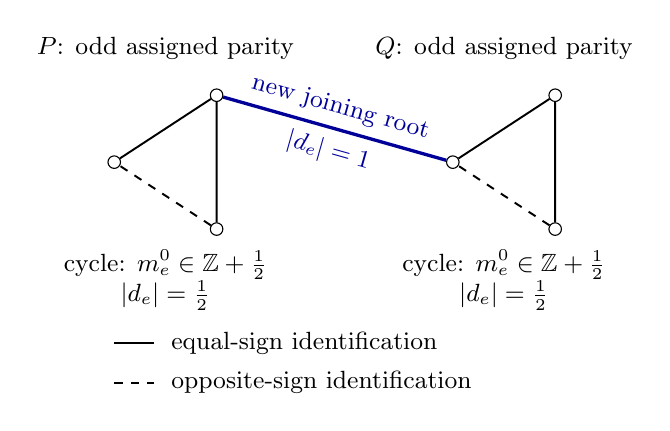
\begin{tikzpicture}[
  x=1cm,y=1cm,
  axis/.style={circle,draw,fill=white,inner sep=1.6pt},
  root/.style={line width=.7pt},
  newroot/.style={line width=1.2pt,blue!60!black},
  every node/.style={font=\small}]
  \node[axis] (p0) at (0,0) {};
  \node[axis] (p1) at (1.3,.85) {};
  \node[axis] (p2) at (1.3,-.85) {};
  \node[axis] (q0) at (4.3,0) {};
  \node[axis] (q1) at (5.6,.85) {};
  \node[axis] (q2) at (5.6,-.85) {};
  \draw[root] (p0)--(p1)--(p2);
  \draw[root,dashed] (p2)--(p0);
  \draw[root] (q0)--(q1)--(q2);
  \draw[root,dashed] (q2)--(q0);
  \draw[newroot] (p1)--node[above,sloped] {new joining root}
    node[below,sloped] {$|d_e|=1$} (q0);
  \node at (.65,1.45) {$P$: odd assigned parity};
  \node at (4.95,1.45) {$Q$: odd assigned parity};
  \node[align=center] at (.65,-1.5)
    {cycle: $m_e^0\in\Z+\tfrac12$\\$|d_e|=\tfrac12$};
  \node[align=center] at (4.95,-1.5)
    {cycle: $m_e^0\in\Z+\tfrac12$\\$|d_e|=\tfrac12$};
  \draw[root] (0,-2.3)--(.5,-2.3);
  \node[anchor=west] at (.6,-2.3) {equal-sign identification};
  \draw[root,dashed] (0,-2.8)--(.5,-2.8);
  \node[anchor=west] at (.6,-2.8) {opposite-sign identification};
\end{tikzpicture}
\caption{The graph underlying the half-relation deformation.
The two original components are unbalanced and have odd assigned
difference parity. A joining root connects their even-sum lattices
inside the full type-$D$ root lattice. For the displayed graph,
half the primitive relation has absolute value $\tfrac12$ on the
cycles and $1$ on the joining edge. More generally the latter
value occurs on the whole connecting path, and coefficients on
other attached trees vanish. Cycle lengths and omitted branches
are schematic; local feasibility is supplied by a local link.}
\label{fig:half-relation}
\end{figure}


\subsection{Sorting collisions and continuing a link}

\begin{proposition}[Continuation]\label{prop:continuation}
Under the standing assumption of no integral schedule, a local link
cannot exist.
\end{proposition}

\begin{proof}
Continuation may replace the ordered root list when times collide.
We therefore follow coefficient lines in a finite set of root lists,
not one fixed list.  Each replacement preserves the endpoint and
transforms the extrapolated coefficients at parameter one by an
integral unimodular change.  First we exclude removable switches at
an interior parameter.  We then use a common potential to select
compatible times for alternative routes through a tied cluster.
The local-link conditions start the motion at parameter zero, and
compactness carries it to parameter one.

\paragraph{Strictness at a continuation point.}
Suppose an exact augmented schedule occurs at a parameter
\(0<s_*<1\), with a primitive half-kernel direction and integral
extrapolation at one.  If a switch is at time zero or one, its
coefficient is integral; a zero-total switch has coefficient zero.
Consequently
\[
 (1-s_*)d_i=m_i(1)-m_i(s_*)\in\Z,
 \qquad |(1-s_*)d_i|<1,
\]
so \(d_i=0\).  Deleting that switch leaves a nonzero relation among
at most \(l\) roots, hence deficient rank.  At an endpoint one may
delete the entire endpoint cluster.  Either operation contradicts
Lemma~\ref{lem:hard-case}.

If a gap is zero, the same reasoning applied to \(G_i\) gives
\(d_i^G=0\), since the extrapolated gap is integral by
\eqref{int:gap}.  Reflect the suffix and delete the switch.  All
remaining velocity roots are unchanged: reflection changes both their
position labels and the accumulated frame by the same factor, which
cancels in \(p_{i-1}^{-1}\beta_i\).  The residual dependence again gives
deficient rank.  Thus all switches at such a parameter are interior,
with strict gaps and totals.

At \(s_*=0\) this arithmetic would not exclude a nonzero half-kernel
entry.  Instead, in an \emph{unaffected} cluster use the forgetting
property of the local link.  Any reordering there preserving its full
reflection product and exact displacement can also be performed after
forgetting the augmentation.  In case \eqref{int:whole-shape}, the same
fixed right stabilizer discrepancy persists after the reordering; in
the reflected-suffix case conjugate the reordered roots back.
One obtains an exact schedule with the original \(l\) switches.
A zero sign or boundary switch could then be removed, leaving at most
\(l-1\) switches, again impossible.  This argument applies after every
successive reordering at that base time.

\paragraph{A common potential at a collision.}
Suppose several candidate times coincide at \(\tau\) when \(s=s_*\).
By Lemma~\ref{int:half-kernel}, throughout that cluster
\begin{equation}\label{int:cluster-potential}
 m_i(s)=\gamma_i\cdot\bigl(-b(\tau)+(s-s_*)L\bigr).
\end{equation}
The candidate time belonging to a root line \(\gamma\) therefore solves
\begin{equation}\label{int:candidate-time}
 \gamma\cdot\bigl(b(t)-b(\tau)+(s-s_*)L\bigr)=0.
\end{equation}
It depends only on that root line and the common potential, not on the
route chosen through the cluster.

Commute an adjacent pair with orthogonal roots whenever its candidate
times are inverted.  For a nonorthogonal pair, the rank-two subsystem
is \(A_2\).  At the base point choose one regular refinement of the
common position order and one of the incoming velocity order,
preserving their strict inequalities, and transport the latter
through the two reflections.  The two steps are decreasing in this
single rank-two Bruhat order.  Both are covers: their length drops
are positive odd integers whose sum is at most three, hence their
sum is two.  Every length-two interval in the \(A_2\) Bruhat order is
a diamond.  Its other route therefore also consists of two downward
covers: the position root is positive, and its inverse image under
the current velocity state is negative, at each step.  Forgetting
the common regular refinements gives weakly correct position and
velocity signs for this other route.
Identical consecutive reflection lines cannot occur, since the first
would reverse the strict velocity inequality required by the second.
Replace the pair by that route with the same product.  The preceding
deletion arguments exclude equality before we require its nearby
inverse times.

The displacement of the pair is unchanged by
\eqref{int:cluster-potential} and the telescoping identity
\eqref{int:telescoping}.  Any two nonparallel roots in this \(A_2\)
subsystem form a basis of its root lattice.  Thus the old and new
coefficient pairs are related by an integral unimodular map.  Outside
the pair the accumulated frame, roots, and coefficients are unchanged.
It follows that the full lattice, the primitive half-kernel direction,
and integral extrapolation at one are all preserved.

\paragraph{Termination of sorting.}
Let \(i,j\) denote the simple root lines of the velocity-positive
system and \(h=i+j\) its remaining root line.  Their candidate times
are \(T_i,T_j,T_h\).  Choose representatives consistently with the
incoming moving order, so that their level functions have the same
strict monotonicity.  Reversing a representative does not change its
candidate-time equation.  The left-hand side of
\eqref{int:candidate-time} for \(h\) is the sum of those for \(i,j\);
strict monotonicity implies that \(T_h\) lies strictly between
\(T_i,T_j\) when they differ.  This holds also across a shape break.
The four possible diamonds, written as successive right reflection
labels in the velocity frame, are
\[
\begin{array}{cc}
\toprule
\text{lengths}&\text{alternative routes}\\ \midrule
3\longrightarrow1&ij\ \longleftrightarrow\ jh\\
3\longrightarrow1&ih\ \longleftrightarrow\ ji\\
2\longrightarrow0&ji\ \longleftrightarrow\ hj\\
2\longrightarrow0&ij\ \longleftrightarrow\ hi.\\
\bottomrule
\end{array}
\]
Indeed, writing \(s_h=s_i s_j s_i=s_j s_i s_j\), their products are
\(s_i s_j=s_j s_h=s_h s_i\) and
\(s_j s_i=s_i s_h=s_h s_j\); the starting length determines which
two factorizations form the interval.  These are the same common
position and velocity refinements used above.
In each row, if the current route is descending in candidate time, the
other route has strictly earlier first time.  For example, in the
first row \(T_i>T_j\) makes the route \(jh\) start earlier; conversely
\(T_j>T_h\) implies \(T_j>T_h>T_i\), so \(ij\) starts earlier.
The other three rows follow by the same between-time inequality.
Orthogonal commutation also strictly decreases the first time of the
inverted pair.

The full candidate-time list therefore decreases lexicographically.
Only finitely many root lists are possible, and each root line has its
fixed candidate time from \eqref{int:candidate-time}.  Sorting
terminates in a weakly ordered list.  All its strict gaps and totals
persist in a common sufficiently small neighborhood of the base
parameter, since there are only finitely many possible lists.
At \(s_*=0\) apply this procedure only to unaffected clusters; the
modified cluster is feasible by the definition of a local link.
Consequently the link gives a genuine schedule for small positive
\(s\).

\paragraph{Arrival at the integral endpoint.}
Consider all parameters in \((0,1]\) admitting an augmented schedule
with \(l+1\) lattice-generating roots, a primitive half-kernel
direction, and integral extrapolation at one.  This set is nonempty by
the preceding paragraph.  Root lists, initial frames, and endpoint
representatives range over finite sets.  The actual coefficients are
bounded by the compact shape, and every direction coordinate has
absolute value at most one.  Their extrapolated integer values at one
are therefore bounded as well and range over a finite set.  The
half-kernel directions themselves also range over a finite set.

At the supremum, choose a subsequence fixing all this discrete data.
The ordered switch times have a convergent subsequence; endpoint
balance and weak signs are closed conditions.  Thus the supremum is
feasible.  If it is less than one, the strictness argument excludes
all boundary or removable switches there, and the common-potential
sorting extends feasibility to its right.  This is impossible.
Parameter one is attained, and every coefficient is then integral,
contrary to the standing assumption.
\end{proof}

The proof only asks for weak order inside a feasible modified cluster.
If two new transfers have the same strictly increasing level function
and equal coefficient derivatives, their times remain exactly equal;
the specified order of simultaneous switches is permitted.

\begin{lemma}[Direct links]\label{lem:direct-links}
In the exceptional schedule with components \(P,Q\), each of the
following produces a forbidden local link:
\begin{enumerate}[label=\textup{(\roman*)}]
\item a signed cross-component pair with strict concordant position
and moving-value orders at time zero;
\item a signed cross-component pair with strict discordant orders at
time one;
\item a position crossing of a cross-component pair with distinct
moving values between old switch times;
\item the crossing in \textup{(iii)} at an old switch time, if both
axes are unused by its cluster.
\end{enumerate}
\end{lemma}

\begin{proof}
In the first case insert the cross swap at time zero, choosing the
initial frame so that the old frame occurs just after the swap.
Before the swap the velocity order is the strict inverse of its
position order, so the gap is positive.  Its coefficient is zero.
The position graph has gained a bridge joining the two odd unbalanced
components; its roots generate the full root lattice.  In the
primitive relation the bridge coefficient has magnitude two.  Indeed,
prune the off-cycle branches and follow the remaining connecting path:
the cycle equations give equal coefficient magnitudes around each odd
cycle, and their sign inconsistency makes the connecting flux twice
that magnitude.  Thus the primitive magnitudes are one on the cycles
and two along the connecting path.  The half-kernel derivative on the
bridge has magnitude one.  Choose its sign to
make the new time move into \((0,1)\).  All old gaps remain positive.
The inserted edge can plainly be forgotten at the exact base time.
The end case is the same construction with the old state before the
new swap; choose the derivative to move its time leftward from one.
Its base coefficient is the integral total root pairing.

For a crossing, insert the swap with its strict approaching inversion
and reflect the entire old suffix.  At the base point its gap is zero,
its total is positive, and continuity holds because the crossing
position is fixed by the reflection.  In the velocity frame all old
roots are retained.  The two component root bases in that frame still
generate their respective even-sum lattices, and the new root is a
bridge between them.  Hence the augmented roots generate \(Q(D_l)\),
and the primitive half-kernel direction in the gap coordinates has
nonzero, indeed unit, coordinate on the bridge.  Choose its sign so
that the new gap becomes positive.  Its time remains interior.
Formula~\eqref{int:gap}, with zero base gap, shows that the inserted
coefficient is half-integral; the other base coefficients remain
half-integral.  Forgetting is precisely reflection of the suffix back.

If the crossing lies at an old cluster unused by its two axes, its new
root is orthogonal to all roots in that cluster.  Commute these
switches to put their nearby candidate times in order.  This proves
local feasibility also in the last case.  Proposition~\ref{prop:continuation}
excludes each construction.
\end{proof}

It remains to show that the exceptional schedule necessarily admits a
link.  Proposition~\ref{prop:strict-count} supplies a strict excess of
cross-component comparisons, while Proposition~\ref{prop:knot-count}
shows that this excess cannot disappear without a locally feasible
link.  These two assertions, proved next, complete
Theorem~\ref{thm:integral-schedule}.

\section{A strict comparison count and simultaneous switches}
\label{sec:moment-knots}

We complete the proof of Theorem~\ref{thm:integral-schedule}.  Work under
its rank induction and suppose, for a contradiction, that no integral
schedule exists.  By Lemma~\ref{lem:hard-case}, the basic schedule has
\(l\) independent switch roots and exactly two components, denoted by
\(P,Q\), both unbalanced and of odd parity.  Every switch has positive
gap, positive total, and an interior time.  The limiting cover property
of Proposition~\ref{prop:basic-schedule} is retained.  Any realization
with fewer than \(l\) switches, or with at most \(l\) switches outside
this exceptional configuration, contradicts Lemma~\ref{lem:hard-case}.
Every feasible extra-edge link contradicts
Proposition~\ref{prop:continuation}.

Write \(\widehat P=\{\pm i:i\in P\}\) and similarly for \(Q\).  For a
signed label \(a\), put \(e_{-a}=-e_a\), \(y_a=y\cdot e_a\), and
\(v_a=(w\mu)\cdot e_a\) in the current frame.  A cross-comparison means
a pair \((a,c)\in\widehat P\times\widehat Q\).  We count each with
weight \(1/2\), so that a comparison and its signed mirror together
have weight one.  Set
\[
 r=2|P|,\qquad h=2|Q|,\qquad R=\frac{rh}{2}.
\]
Let \(p_\lambda,p_\mu,p_\xi\) be the numbers, with this same weight,
of cross ties in the initial positions, assigned moving values, and
final positions.  The middle number is independent of the time at
which the assigned values are read.

\subsection{The strict moment inequality}

Our aim is the strict inequality \(R>p_\lambda+p_\mu+p_\xi\).
The moments on the two components turn its tie counts into spectral
multiplicity counts.  For a Hermitian triple on \(\C^r\), its
\emph{profile} is the collection
\(m=(m_i(a))_{i,a}\), where \(m_i(a)\) is the multiplicity of the
numerical eigenlevel \(a\) of its \(i\)-th member.  Absent levels have
multiplicity zero.  Profiles of different sizes are compared using
the same three sets of numerical levels.

Writing \(m^P,m^Q\) for the profiles of the component moments, we
will have \(p_\lambda+p_\mu+p_\xi=(m^P\cdot m^Q)/2\).
An orbit-dimension estimate will give the required weak bound by
Cauchy--Schwarz, with a separate treatment of a moving zero level.
Without that zero, equality forces proportional profiles of full
norms \(r,h\).  We will also establish irreducibility in this equality
case, so the next lemma forces the two sizes to agree.  In the proof
of strictness, identical profiles will yield a forbidden permutation
block.

The lemma's direct-sum argument is a flag formulation of the
canonical-decomposition methods for quiver representations developed
by Kac and Schofield \cite{Kac1982,Schofield1992}. We give it directly
in terms of the three spectral filtrations.

\begin{lemma}[Profile rigidity]\label{knot:profile-rigidity}
Suppose two irreducible Hermitian zero-sum triples have proportional
profiles \(m,m'\), of sizes \(r,h\), respectively, and
\[
 \|m\|^2=r^2,\qquad \|m'\|^2=h^2.
\]
Then \(r=h\) and \(m=m'\).
\end{lemma}

\begin{proof}
\emph{Flags with scalar endomorphisms.}
For a profile \(m\), let \(\mathcal F(m)\) be the product of the three
partial-flag varieties with the prescribed upper-level dimensions.
Its complex dimension is
\begin{equation}\label{knot:flag-dimension}
 \dim_\C\mathcal F(m)
 =\frac{3r^2-\|m\|^2}{2}=r^2.
\end{equation}
The product of the corresponding Hermitian orbits has real dimension
\(2r^2\).  At an irreducible zero-sum triple, the sum map is submersive
onto the traceless Hermitian matrices: the orthogonal cokernel consists
of common commuting Hermitian matrices, which are scalar.  Its local
zero-sum fiber therefore has dimension \(r^2+1\), whereas simultaneous
unitary conjugation has orbit dimension \(r^2-1\).  Irreducibility is
open.  It follows that these fixed spectra admit arbitrarily many
pairwise unitarily inequivalent irreducible zero-sum triples.

Their upper-level flags have scalar endomorphisms, and flags from two
inequivalent triples have no nonzero morphism.  Indeed, let \(L\)
preserve all three upper-level filtrations, from a triple \((X_i)\)
to a triple \((X'_i)\).  In spectral coordinates its nonzero matrix
entries go from a level \(a\) only to levels \(a'\ge a\).  Consequently
\[
 \tr(L^*X'_iL-L^*LX_i)
   =\sum_{a,a'}(a'-a)\|L_{a',a}\|^2\ge0.
\]
The sum of these three quantities is zero.  Thus every nonzero entry
has \(a'=a\), and \(X'_iL=LX_i\) for all \(i\).  Irreducibility now
gives the assertions.  Here an invertible complex intertwiner between
irreducible Hermitian triples is a scalar multiple of a unitary
intertwiner, since \(L^*L\) commutes with the source triple.

\emph{Direct sums fill an open set.}
The Hermitian triples have supplied Hom-free spectral flags.  We now
work in the complex flag varieties: the configurations in the
direct-sum families need not themselves arise from Hermitian
zero-sum triples.  For every positive integer \(b\), direct sums of
\(b\) configurations in \(\mathcal F(m)\) having scalar endomorphisms, with arbitrary
changes of frame, contain a nonempty Zariski-open subset of
\(\mathcal F(bm)\).  To prove this, choose \(b\) pairwise Hom-free
configurations as above and examine the differential of the direct-sum
map, including the action of \(\GL(br,\C)\).  The flag tangent space
splits into ordered blocks indexed by the summands.  Its diagonal
blocks are supplied by variation of the individual flags.  Each
off-diagonal ordered block has dimension \(r^2\): the contribution
of its \(i\)-th flag is
\[
 \sum_{a<b}m_i(a)m_i(b)
 =\frac{r^2-\sum_a m_i(a)^2}{2},
\]
and summing gives \eqref{knot:flag-dimension}.  Change of
frame maps a space of \(r\times r\) matrices to that block; its kernel
is exactly the space of filtration-preserving maps between the two
summands, which is zero.  Hence this differential is surjective.
The direct-sum map is therefore dominant.  Chevalley's theorem makes
its image constructible \cite[Tag~054K]{StacksProject}; a dense
constructible subset of an irreducible variety contains a nonempty
Zariski-open subset.  Requiring scalar
endomorphisms on the summands is an open condition and includes our
chosen point, so the same assertion holds with this requirement.

We finish with the scalar-endomorphism case of the Krull--Schmidt
uniqueness argument; compare \cite[Theorem~1]{Atiyah1956}.
Choose positive integers \(b,b'\) with \(bm=b'm'\).  The two nonempty
open subsets just obtained intersect in the irreducible variety
\(\mathcal F(bm)\).  One configuration in their intersection admits
two direct-sum decompositions
\[
 V=\bigoplus_i V_i=\bigoplus_j W_j,
\]
whose summands have scalar endomorphisms, with dimensions \(r\) and
\(h\), respectively.  Inclusions and projections preserve all three
flags.  On a fixed \(V_i\), the sum of the composites
\(V_i\to W_j\to V_i\) is the identity.  One composite is therefore
a nonzero scalar.  Write it as \(gf=c\,\mathrm{id}_{V_i}\), \(c\ne0\).
The endomorphism \(fg\) of \(W_j\) is also scalar, and
\((fg)f=cf\) shows that its scalar is \(c\).  Thus \(f\) is an
isomorphism, so \(r=h\).  Proportional profiles of equal size are equal.
\end{proof}

\begin{proposition}[Strict comparison count]\label{prop:strict-count}
In the standing exceptional configuration,
\begin{equation}\label{knot:strict-count}
 C:=R-p_\lambda-p_\mu-p_\xi>0.
\end{equation}
\end{proposition}

\begin{proof}
Choose skew-symmetric zero-sum triples from the separate moment
solutions in \(P\) and \(Q\), supplied by
Lemma~\ref{lem:schedule-moment}.  Let \(m^P,m^Q\) be the profiles of
\(i\) times these triples.  Since the spectra of a real skew matrix
occur in opposite pairs,
\begin{equation}\label{knot:profile-ties}
 p_\lambda+p_\mu+p_\xi=\frac{m^P\cdot m^Q}{2}.
\end{equation}
A common nonzero skew operator commuting with either triple would give
a forbidden splitting by Lemma~\ref{lem:block-reduction}.  Thus both
common skew stabilizers vanish.

\emph{The norm bound.}
Consider one block of real dimension \(r\), write its matrices as
\(A_1,A_2,A_3\), and put \(z_i=\dim\ker A_i\).  For one matrix, a
kernel of dimension \(z_i\) contributes \(z_i(z_i-1)/2\) to its skew
stabilizer; a positive rotation level of multiplicity \(k\) contributes
\(k^2\).  The squared profile norm instead has contributions \(z_i^2\)
and \(2k^2\).  Hence twice the sum of the three stabilizer dimensions
is \(\|m\|^2-\sum_i z_i\).  The orbit sum map is submersive onto
\(\mathfrak{so}(r)\), because its orthogonal cokernel is the common
skew stabilizer.  Its kernel contains the simultaneous-conjugation
tangent, of dimension \(\dim\SO(r)\).  Comparing dimensions gives
\begin{equation}\label{knot:profile-bound}
 \|m\|^2-\sum_i z_i\le r^2-r.
\end{equation}

If the joint kernel is zero, the map
\[
 u\longmapsto(A_1u,A_2u,A_3u)
\]
is injective into the kernel of addition from
\(\bigoplus_i\im A_i\) to \(\R^r\).  This addition map is onto:
the orthogonal complement of the sum of the images is the joint
kernel.  Its kernel has dimension \(2r-\sum_i z_i\), so
\(\sum_i z_i\le r\).  Equation~\eqref{knot:profile-bound} yields
\(\|m\|\le r\).  The same proof works in odd dimension.

A joint kernel of dimension at least two would support a nonzero
commuting skew operator.  A possible joint kernel is therefore a
single line, and it must belong to the block containing the sole
possible zero of the moving weight.  Remove this line.  The reduced
triple has neither a joint kernel nor a common skew stabilizer, so
\[
 \|m\|^2
 =\|m_{\mathrm{red}}\|^2+2\sum_i z_{i,\mathrm{red}}+3
 \le(r-1)^2+2(r-1)+3=r^2+2.
\]
The moving zero-level entry in the original profile has multiplicity
two and pairs with zero in the other block's profile.  Deleting that
entry for the dot product improves the relevant squared bound to
\(r^2-2\).  Cauchy--Schwarz is then strict.  If there is a moving zero
but no joint kernel, the bounds \(\|m^P\|\le r\),
\(\|m^Q\|\le h\) are already strict in Cauchy--Schwarz, since the
moving zero entry prevents proportionality.  Thus
\(m^P\cdot m^Q<rh\) whenever the moving weight has a zero.

\emph{Excluding equality without a moving zero.}
The weak bound \(m^P\cdot m^Q\le rh\) holds by the same estimates.
Equality forces proportional profiles, \(\|m^P\|=r\),
\(\|m^Q\|=h\), and \(\sum_i z_i=r\) in the first block, with the
analogous equality in the second.  The moving matrices are invertible.
Each of the other two matrices has a kernel: if one were invertible,
the other would vanish, and the remaining pair \(A,-A\) would have
\(A\ne0\) in its common skew stabilizer.

Both triples are absolutely irreducible.  Indeed a proper common real
invariant subspace has an invariant orthogonal complement.  Each has
even dimension, since the moving restriction is invertible and skew.
Together with the other original block this gives at least three
orthogonal blocks, contrary to Lemma~\ref{lem:block-reduction}.  A
proper complex invariant subspace for the Hermitian triple gives a
nonscalar commuting Hermitian projection \(B+iD\), with \(B\) real
symmetric and \(D\) real skew.  Both commute with the real skew triple.
A nonscalar \(B\) gives the forbidden real splitting, while nonzero
\(D\) gives the forbidden skew stabilizer.

Lemma~\ref{knot:profile-rigidity} now gives \(r=h\) and identical
profiles, including their numerical levels.  Replace the second skew
triple by an orthogonal copy of the first.  Choose the isometry's
orientation to match the moving special-orthogonal orbit.  The other
two matrices impose no additional orientation restriction: each has a
kernel, and reflection in a kernel line is an orientation-reversing
commuting isometry.  Thus their orthogonal and special-orthogonal
orbits coincide.  On the sum of the two isometric copies, the skew
operator rotating one copy into the other commutes with the triple.
It gives a unitary, hence permutation-type, block in
Lemma~\ref{lem:block-reduction}, again a contradiction.  Equality is
impossible.  Equation~\eqref{knot:profile-ties} proves
\eqref{knot:strict-count}.
\end{proof}

\subsection{Core phases and the comparison function}

The moment calculation has produced the strict numerical gap
\(R-p_\lambda-p_\mu-p_\xi>0\). We now follow the cross-component
comparisons along the schedule. Strict inversions alone do not record
what happens on an interval where both positions and moving values
agree. The phases defined next provide the correction for these
double ties: such an interval will contribute \(-1\) when its two
phases are zero and \(+1\) when they are one.  The phase restriction
is a consequence of the exceptional graph, not an arbitrary choice
of a tie-breaking order.

For a signed position label \(a\), define its \emph{core phase}
\(p_a(t)\) on the open intervals between switch times.  If its axis is
off the unique cycle of its component, its phase is zero until the
switch on the first edge toward that cycle and one afterward.  If its
axis lies on the cycle, its phase is \(0,\tfrac12,1\), according as
zero, one, or two of its cycle incidences have occurred.  The phase is
unchanged on replacing \(a\) by \(-a\).

There is a useful algebraic description.  Solve the component's
root-basis equation with right-hand side \(e_a\).  The cumulative
signed \(a\)-coordinate of the edges already used is \(p_a(t)\).
For an off-cycle source, pruning the attached trees leaves a unit
contribution on its first edge toward the cycle.  At a cycle source,
the two incident cycle contributions are each one half.  This proves
the description.  Since the actual coefficients are integral on
bridges and half-odd-integral on cycle edges, phase \(1/2\) also records
that the translation term in the position formula has changed its
fractional part by a half.

\begin{lemma}[Plateaus]\label{lem:plateau}
Suppose cross labels \(a,c\) have equal position and equal assigned
moving value on an open interval between switch times.  Then
\begin{equation}\label{knot:plateau-phases}
 (p_a,p_c)=(0,0)\quad\hbox{or}\quad(1,1).
\end{equation}
\end{lemma}

\begin{proof}
The equality of moving values on distinct axes means that their
assigned shape-coordinate forms agree on the whole minimal chamber
face.  Hence their shape values agree for every time.  The initial
coordinates have the same fractional part, and equality of the current
positions implies that either both phases are half or neither is.

At any point of the plateau, reflect the entire suffix by the
reflection exchanging the two signed axes, including every later
position and switch root.  This reflection fixes the position at the
cut and fixes the current-frame shape \(w\eta(t)\) for every \(t\),
since the two coordinate forms agree.  Thus no new switch is needed
at the cut, and the reflected endpoint remains in its original Weyl
orbit.  In the root graph, cut each involved
vertex into its past and future copies, then identify opposite-time
copies crosswise.  If both phases are half, each cut opens its cycle
into a connected tree.  The crosswise identification gives a connected
\(l\)-edge graph, outside the exceptional configuration.  If neither
phase is half, one cut piece contains the cycle and the other is a
tree, possibly an isolated vertex.  The core piece uses the past copy
at phase one and the future copy at phase zero.  Opposite phases
therefore join the two cores and leave a separate tree component.
That too is excluded by Lemma~\ref{lem:hard-case}.  Only
\eqref{knot:plateau-phases} remains.
\end{proof}

For times between events, define
\begin{equation}\label{knot:J-definition}
 J(t)=\frac12\sum_{a\in\widehat P,\ c\in\widehat Q}j_{a,c}(t),
 \qquad
 j_{a,c}(t)=
 \begin{cases}
  1,&(y_a-y_c)(v_a-v_c)<0,\\
  p_a+p_c-1,&y_a=y_c\ \hbox{and}\ v_a=v_c,\\
  0,&\text{otherwise}.
 \end{cases}
\end{equation}
Use one-sided values at isolated equalities.  The direct links of
Lemma~\ref{lem:direct-links} give
\begin{equation}\label{knot:J-boundaries}
 J(0+)\ge R-p_\lambda-p_\mu,
 \qquad J(1-)\le p_\xi.
\end{equation}
Indeed strict position and velocity orders must begin discordant and
end concordant.  An initial double tie has phases zero and contributes
\(-1\), covered by subtracting both sorts of initial tie.  At the
final endpoint a double tie has phases one and contributes \(+1\);
a position tie with distinct velocities is an inversion just before
the endpoint and is also counted by \(p_\xi\).  Away from the old
switch times, any changing cross equality with distinct velocities
gives the direct crossing link.  Thus a decrease can occur only at an
old switch time, which we call a \emph{knot}.

\begin{proposition}[Monotonicity at knots]\label{prop:knot-count}
Under the standing no-integral-schedule assumption, the function
\(J\) is nondecreasing at every knot, and hence on the whole interval
in the one-sided sense used above.
\end{proposition}

We prove this by reducing each knot to disjoint transfers of two
moving values.  A loss in their strict comparison count will either
produce a local link or be compensated by a double-tie contribution.

\subsection{The form of an exact knot}

We now specify the shape genericity allowed by
Lemma~\ref{int:closedness}.  This choice concerns the original
exceptional root-basis schedule, which retains the limiting cover
property; it imposes no cover condition on later augmented schedules.
For fixed endpoint assignments and a fixed root basis, the endpoint
equation determines every coefficient.  The frames, coefficients,
and translation parts therefore range over finitely many possibilities.
Both switch conditions and equalities of signed positions consequently
give a finite collection of affine level sets for shape values.

Let \(F\) be the span of the smallest chamber face containing \(\mu\).
Its signed coordinate forms are \(\pm M_j\), for independent
variables \(M_j\), with possible repetitions.  No coordinate form
is forced to vanish: a sole zero coordinate of \(\mu\) is the free
last coordinate in type \(D\).  On distinct axes, any equality at
\(\mu\) already identifies the corresponding forms on \(F\).

Choose a polygonal shape, with slopes relatively interior in the face,
that avoids simultaneous nonconstant affine level hits having
nonproportional restrictions to \(F\), and avoids such hits at its
breaks.  Such choices are dense: after subdivision, interior break
values have open freedom in \(F\), and a generic polygonal path
avoids the finitely many affine sets of codimension at least two.

At any knot the nonzero velocity differences of its switches are
therefore multiples of one form \(\ell\).  Group signed position labels
by their assigned forms modulo \(\R\ell\).  This partition is unchanged
during the knot.  If \(\ell\) is proportional to \(M_i\pm M_j\),
\(i\ne j\), its nontrivial classes are pairs of forms and their
mirrors.  If it is proportional to \(M_i\), the only nontrivial class
is \(\{M_i,-M_i\}\).  Consequently each class has either one value or
two values \(H>L\), ordered at \(\mu\).  The sole possible exception,
\(M_i(\mu)=0\) in an opposite class, contains only the two signs of
one physical axis; it supports no root switch and may be omitted.

Across different classes, cross positions are unequal at the knot
and cross velocity values are distinct.  A swap changes their strict
inversion count only if an external spectator lies strictly between
both swapped positions and both swapped velocity values.  The
limiting cover property excludes exactly this situation by
Corollary~\ref{real:blocker}.  Thus these
comparisons are unchanged.  Classes with one value need only the
monotonicity of phases.

\begin{lemma}[Matching at a knot]\label{knot:matching}
Within each two-value class at a knot, the transfers of the high value
form disjoint matching pairs inside each component, together with
unused single labels.  In an opposite class the matching is disjoint
on physical axes, with its mirror transfers understood as the same
physical switches.
\end{lemma}

\begin{proof}
Every transfer sends \(H\) from a donor of lower position to a
recipient of higher position.  In an ordinary class, decompose this
flow into directed paths from its net donors to its net recipients.
Positions strictly increase, so no directed cycle occurs.  Shortcut
each path by its direct transfer.  The resulting matching has the
same final high and low assignments and legal positive gaps; see
Equation~\eqref{int:whole-shape}.  If the
original transfers were not already disjoint pairs, this uses fewer
switches, contrary to Lemma~\ref{lem:hard-case}.

In an opposite class each physical swap flips two axes, producing two
mirrored transfers.  Mark each axis by its initial high sign.  At any
edge occurrence, the sum of the positions in the two \emph{currently}
high signs is strictly negative.  At each vertex, pair consecutive
incidences, leaving the first unpaired if their number is odd.  The
signed-position terms in each such pair cancel, because the high sign
alternates.  The paired incidences organize the edges into paths and
cycles.  A cycle would sum strict inequalities to \(0<0\), and cannot
occur.  On a path the sum leaves just the positions of its two ends
in their initial high signs, with negative sum.  A direct flip of
these two axes is therefore feasible.  Distinct paths have disjoint
unpaired ends; their flips realize exactly the original odd-incidence
axes, hence exactly the same final sign assignment.  Unless the old
switches were already physically disjoint, this again reduces their
number.
\end{proof}

We may therefore compare units---single labels and directed pairs---of
one component with units of the other.  All local replacements below
use distinct physical axes.  Other switches at the knot are disjoint
from these axes, apart from the automatic mirrors in an opposite
class.  A transfer \(a\to b\) has root \(e_b-e_a\); all transfers in
the same two-value class have the same strictly increasing coefficient
function, namely the assigned shape value of \(H\) minus that of \(L\).

The replacements have exactly the same final assignment of \(H,L\)
as the old switches.  This preserves the whole shape, not merely its
value at the knot: the old and new final frames differ on the right
by an element of \(W_\mu\), which fixes \(F\) pointwise.  Subsequent
switches therefore have the same actual shape values and positions
at the base parameter.  The forgetting condition of
Proposition~\ref{prop:continuation} is satisfied.  We will check its
remaining hypotheses---lattice generation and feasible coefficient
order and gaps---for each extra-edge replacement.

\subsection{Pairs, single labels, and endpoint ties}

The matching lemma leaves three kinds of comparison: two unused
labels, a transfer and an unused label, and two transfers. We check
that every decrease either produces a link or is offset by the
contribution of a double tie.

Consider a transfer \(a\to b\) at positions \(x<z\), and a single
label \(c\) in the other component at position \(h\), initially high.
The low case is obtained by taking signed mirrors.  Omitting plateau terms, the strict count
decreases by one precisely when
\begin{equation}\label{knot:pair-single-overlap}
 x\le h\le z.
\end{equation}
Indeed before the knot only the comparison of \(c\) with the low
recipient can contribute; afterward only its comparison with the
new low donor can contribute.  At an endpoint equality, the distinct
approaching or departing velocities give respectively the inversion
or concordance specified by the closed inequalities in
\eqref{knot:pair-single-overlap}.

Replace the transfer by
\begin{equation}\label{knot:split}
 c\longrightarrow b,\qquad a\longrightarrow c.
\end{equation}
The final high value is at \(b\), as required.  The graph subdivides
the old edge through the other component, with the same cycle signs;
it is connected and unbalanced and generates the full root lattice.
Its base coefficients are the common old coefficient, hence
half-integral.  Let \(d_1,d_2\) be the derivatives of its two new
coefficients under a primitive half-kernel direction.  Their difference
\[
 D=d_2-d_1
\]
is nonzero: otherwise contracting the two new edges would give a
dependency of the old basis.  Choose its sign so that \(D>0\).
The common increasing coefficient function then orders the two new
times correctly.  If \(x<h<z\), both gaps are strictly positive and
\eqref{knot:split} is a forbidden feasible link.

It remains to compute the derivative of a zero gap.  For an ordered
switch root \(\beta_i\), use Equation~\eqref{int:gap}.
The two new roots are
\(\beta_1=e_b-e_c\), \(\beta_2=e_c-e_a\), with
\(\beta_1\cdot\beta_2=-1\).

\emph{A tie at the donor.}
If \(h=x\), the second new gap is zero.  Since the old root is
\(\beta_1+\beta_2\), write
\[
 d_1\beta_1+d_2\beta_2
 =d_1(\beta_1+\beta_2)+D\beta_2.
\]
The full derivative has zero root sum.  Absorbing \(d_1\) into the
old edge therefore gives an old-basis equation with right-hand side
\(-D\beta_2=D(e_a-e_c)\).  By the algebraic description of phases, its
pre-knot contributions at \(a,c\) are \(Dp_a^-,-Dp_c\).
Differentiating \eqref{int:gap}, including the first new
switch, gives
\begin{equation}\label{knot:donor-gap}
 G'_2=D(p_a^-+p_c)+d_1-d_2
      =D(p_a^-+p_c-1).
\end{equation}
Before the knot, \(a,c\) form a double plateau.  If both phases are
one, \eqref{knot:donor-gap} is positive and gives a feasible link.
Otherwise Lemma~\ref{lem:plateau} makes both phases zero.  Losing the
plateau contribution \(-1\) then compensates for the strict-count
loss of one.

\emph{A tie at the recipient.}
If \(h=z\), the first new gap is zero.  This time write the new
derivative as \(d_2(\beta_1+\beta_2)-D\beta_1\).
Absorbing \(d_2\) into the old edge gives right-hand side
\(D\beta_1=D(e_b-e_c)\) in the old-basis equation.  At the old edge,
its contribution to the \(b\)-coordinate is \(d_2\), so
\(p_b^+=p_b^-+d_2/D\).  Equation~\eqref{int:gap} gives
\begin{equation}\label{knot:recipient-gap}
 G'_1=-D(p_b^-+p_c)-d_1
      =D(1-p_b^+-p_c).
\end{equation}
The ensuing plateau of \(b,c\) has either two zero phases, giving
a feasible link, or two unit phases.  In the latter case its new
contribution \(+1\) compensates for the strict loss.  Thus every
pair--single comparison is nondecreasing when links are excluded.
Two singles can decrease only by a crossing with distinct velocities.
Their axes are unused by the knot, so this is a direct link by
Lemma~\ref{lem:direct-links}.

\subsection{Two pairs and the star replacement}

Consider \(a\to b\) at positions \(x<z\) and \(c\to d\) at
positions \(h<k\).  Before the knot the two mixed comparisons count
when \(x\le k\) and \(h\le z\); after it they count when \(x>k\)
and \(h>z\).  Thus, without plateau terms, the loss is two precisely
when the closed intervals \([x,z]\), \([h,k]\) overlap, and zero
otherwise.  The endpoint convention again follows from one-sided
times.  For example, if \(x=k\), the high donor \(a\) lies just below
the low recipient \(d\) before the knot, giving an inversion; after
the knot the same position order is concordant with their exchanged
values.

A touching mixed endpoint permits the switched matching
\[
 a\longrightarrow d,\qquad c\longrightarrow b
\]
with a zero gap and the correct other weak signs.  Deleting that
zero-gap switch leaves fewer than \(l\) edges.  Suppose henceforth
that the overlap is strict.  The two old coefficients are equal.
If they are half-odd-integral, both edges lie on their components'
cycles.  Switching the matching joins the two opened cycles into a
connected \(l\)-edge graph, again outside the exceptional
configuration.  It is immaterial whether the resulting connected
graph is balanced: a balanced graph gives the permutation reduction.

The remaining case has integral common coefficient.  Both old edges
are bridges.  For each bridge, say that its \emph{core is at an
endpoint} if the piece containing that endpoint after removal of the
bridge contains the cycle.  This switch advances the phase from zero
to one at the endpoint away from the core and leaves the core-side
endpoint phase unchanged.

Suppose the donor positions differ, say \(x<h\).  Use the star at
\(c\): send \(c\) to one of \(b,d\), then \(a\) to \(c\), then
\(c\) to the other of \(b,d\).  Strict overlap implies that all three
gaps are positive.  The new graph joins the four pieces of the two
removed bridges by this star.  It is connected, retains both
unbalanced cycles, and generates the full root lattice.  Along the
path between its two cores, the primitive half-kernel coefficients
have magnitude one; off that path the connecting-tree coefficients
vanish.  In the displayed root orientations, their possibilities are
as follows, up to reversing their common sign:
\begin{center}
\begin{tabular}{@{}ccc@{}}
\toprule
Core endpoints & \((d_{c\to b},d_{a\to c},d_{c\to d})\)
 & Wing order feasible?\\
\midrule
\(a,c\) & \((0,1,0)\) & no\\
\(a,d\) & \((0,1,1)\) & yes\\
\(b,c\) & \((1,0,0)\) & yes\\
\(b,d\) & \((1,0,-1)\) & yes\\
\bottomrule
\end{tabular}
\end{center}
To see the signs directly, only the star edges on the path from the
first core endpoint to the second are active.  Conservation at
\(c\) gives equal coefficients on \(a\to c,c\to d\), and opposite
coefficients on \(c\to b,c\to d\).  This gives exactly the table.
All three coefficients use the same increasing shape-level function.
One can therefore order the wings so that their derivatives surround
the middle derivative except when both cores are at donors.  Equal
derivatives give equal times, with the stated switch order at that
time.  In every other case this is a feasible link.

For a receiver star, if \(z<k\), use
\[
 a\longrightarrow b,\qquad b\longrightarrow d,\qquad
 c\longrightarrow b,
\]
allowing the two wing transfers into \(b\) to be interchanged.
Strict overlap makes all gaps positive.  The wing derivatives are
those of \(a\to b\) and \(c\to b\); they must bracket the middle
derivative on \(b\to d\).  If the cores are at \(b,d\), only the
middle edge lies on the path between them, so its nonzero derivative
cannot be bracketed by the two zero wing derivatives.  In every
other case, the active path uses the two wings with opposite
derivatives, the middle and one wing with equal derivatives, or one
wing alone with the other two derivatives zero.  Choosing the common
sign and the wing order makes the times weakly increasing.  Thus
only the case of two recipient cores is infeasible.  If \(k<z\),
interchange the two original pairs.

If no link exists, the donor-star and receiver-star obstructions
cannot both hold.  Thus \(x=h\) or \(z=k\), or both.  These
same-role coincidences produce double plateaus on both sides of the
knot.  If only the donors coincide, the receiver star forces both
cores to be at recipients.  Each donor phase then jumps from zero
to one, so their plateau contribution rises from \(-1\) to \(+1\).
This compensates for the strict-count loss of two.  If only the
recipients coincide, the donor star forces both cores to be at
donors, and the same compensation occurs at the recipients.  If both
pairs of endpoints coincide, the sum of the two plateau increments
is two by the bridge-phase rule, again the required compensation.  This exhausts all pair--pair
comparisons.  Mirrored transfers give the same calculations; the
factor \(1/2\) in \eqref{knot:J-definition} applies uniformly.

\begin{proof}[Proof of Proposition~\ref{prop:knot-count}]
Comparisons across distinct form classes are unchanged by the cover
property.  Within a class, Lemma~\ref{knot:matching} reduces all
comparisons to the single--single, pair--single, and pair--pair cases
just proved.  Each possible loss either gives a feasible extra-edge
link, forbidden by Proposition~\ref{prop:continuation}, or is
compensated by its plateau contribution.  The direct crossing links
exclude decreases away from knots.  Summing gives the assertion.
\end{proof}

\begin{proof}[Completion of the proof of Theorem~\ref{thm:integral-schedule}]
Proposition~\ref{prop:strict-count} and
\eqref{knot:J-boundaries} imply \(J(0+)>J(1-)\), contradicting
Proposition~\ref{prop:knot-count}.  This proves integral realizability
for the generic shapes used above.  The uniform bounded-switch
closedness of Lemma~\ref{int:closedness} passes to an arbitrary shape
with the same endpoint.  Together with the permutation case and the rank
reduction of Lemma~\ref{lem:hard-case}, this completes that theorem.
\end{proof}

\section{From integral schedules to tensor intertwiners}
\label{sec:columns}

The switch integrality in Definition~\ref{def:schedule} is weaker than
the usual integral saturated-chain condition in a highest-weight path
model.  We now prove the representation-theoretic implication that is
needed here directly, using fundamental columns.

\begin{proposition}[Column intertwiners]\label{prop:columns}
Let $\lambda,\mu,\xi$ be dominant integral weights of type $D_n$,
$n\ge2$.  Choose a shape obtained by concatenating straight segments
whose increments are fundamental weights and whose sum is $\mu$.
If this shape admits an integral schedule from $\lambda$ to $W\xi$,
then
\[
 \Hom_G\bigl(V(\lambda)\otimes V(\mu),V(\xi)\bigr)\ne0.
\]
An empty list of columns is allowed when $\mu=0$.
\end{proposition}

We first record carefully what happens to integrality when a schedule
is folded into the dominant chamber.

\begin{lemma}\label{col:folding}
An integral schedule can be folded into a dominant path with Weyl
direction states in decreasing Bruhat order.  Its changes of state
can be expressed as an ordered sequence of downward reflections,
including at coincident times.  At each such step, from $w$ to
$s_\alpha w$ at time $t$,
\begin{equation}\label{col:folded-integrality}
 \alpha\cdot w\eta(t)\in\Z.
\end{equation}
For a concatenation of fundamental columns, all column endpoint
positions of the folded path are dominant integral weights.
\end{lemma}

\begin{proof}
Use the simplifications and folding construction in the proof of
Lemma~\ref{lem:schedule-moment}.  After deleting removable switches,
perturb the remaining strict schedule to separate its sites and make
ordinary chamber crossings transverse.  In the perturbed path, an
original switch becomes a downward reflection in the current chamber
frame, and a sorting crossing becomes a downward simple reflection.
There are at most the longest Weyl length many such strict downward
steps.  Taking a subsequence fixes their discrete labels and order;
their times then converge.  This gives the asserted ordered chain even
if several steps acquire the same limiting time.  The perturbations
used for this construction need not be integral.

Integrality is checked on the limiting chain, in its specified order.
For an original switch, changing the chamber frame changes both its
root and its direction by the same Weyl element.  Its pairing in
\eqref{col:folded-integrality} is therefore the original integral
pairing.  For a sorting crossing, suppose all preceding coefficients
are integral and write the position before that crossing as
\begin{equation}\label{col:prefix}
 x=\lambda+w\eta-\sum_{j< i}m_j\beta_j.
\end{equation}
The wall equation $\alpha\cdot x=0$ gives
\[
 \alpha\cdot w\eta
 =-\alpha\cdot\lambda
   +\sum_{j<i}m_j\,\alpha\cdot\beta_j\in\Z.
\]
The usual switch identity preserves \eqref{col:prefix} after the
crossing.  Induction therefore proves integrality for every prefix,
also inside a limiting cluster.  At a column endpoint $\eta$ is a
weight, so \eqref{col:prefix} shows that $x$ is a weight.  It is
dominant by construction.
\end{proof}

Consider a single column of weight $\omega$.  Normalize its parameter
to $0\le\tau\le1$, so that the original shape on this interval is
$\chi+\tau\omega$, with $\chi$ a sum of preceding fundamental
weights.  Write $x_0,x_1$ for its dominant endpoints and put
$\delta=x_1-x_0$.  Let $u$ and $v$ be the first and last Weyl states
in its open interior.  Boundary-time steps are left between the
columns; thus the last state of one column dominates the first state
of the next.  Since $\alpha\cdot w\chi$ is integral,
Lemma~\ref{col:folding} gives at every interior step
\begin{equation}\label{col:local-level}
 \tau\,\alpha\cdot w\omega\in\Z.
\end{equation}

\paragraph{Minuscule columns.}
For a minuscule weight, all root pairings are $0$ or $\pm1$.
Consequently \eqref{col:local-level} permits no interior reflection
that changes $w\omega$.  The column is straight, with
$\delta=u\omega$.  The extremal case of
Lemma~\ref{lem:coefficient} gives an intertwiner
\[
 V(x_0)\otimes V(\omega)\longrightarrow V(x_1)
\]
whose highest-to-highest coefficient is nonzero at the fixed flag $u$.
This includes the vector column and both spin columns.  For $D_2$
and $D_3$ all fundamental columns are minuscule.
The classical exterior and half-spin models are described in
\cite[Lectures~19--20]{FH91}; here only their root-pairing property
is needed for the minuscule case.
Although full Weyl states inside the column may change while fixing
$\omega$, this causes no problem for composition: the chosen fixed
waypoint has future $u$, and $u\ge v$ dominates the next column's
initial state.

It remains to treat an exterior column
\[
 \omega=e_1+\cdots+e_k,\qquad 2\le k\le n-2.
\]
Let $E$ be the standard $2n$-dimensional quadratic space, with basis
$E_{+i},E_{-i}$ satisfying
$(E_{+i},E_{-j})=\delta_{ij}$ and all other basis pairings zero.
The module $\bigwedge^k E$ is the fundamental module $V(\omega)$;
its flag vectors are wedges of isotropic $k$-planes.

\paragraph{The coefficient to be constructed.}
For the exterior column, Lemma~\ref{lem:coefficient} reduces the
intertwiner problem to a functional supported at weight $\delta$.
The following criterion isolates its annihilation conditions. We will
then construct such a functional and a flag at which it is nonzero,
with past and future limits $u,v$ so that columns can be composed.

\begin{lemma}\label{col:common-walls}
Let $J$ be the set of simple roots $\alpha_i$ with
$x_0\cdot\alpha_i=x_1\cdot\alpha_i=0$.
A functional supported on the weight space of weight $\delta$ in
$\bigwedge^k E$, invariant under the semisimple group generated by
$J$, is an allowed highest-to-highest coefficient for an intertwiner
$V(x_0)\otimes V(\omega)\to V(x_1)$.
\end{lemma}

\begin{proof}
Put $h_i=x_0\cdot\alpha_i$ and $h'_i=x_1\cdot\alpha_i$.
By Lemma~\ref{lem:coefficient}, the functional must annihilate
$f_i^{h_i+1}V(\omega)$ for every $i$.  A vector contributing to its
weight-$\delta$ component would have source weight
$\delta+(h_i+1)\alpha_i$, whose simple-root pairing is
\[
 \bigl(\delta+(h_i+1)\alpha_i\bigr)\cdot\alpha_i
 =h_i+h'_i+2.
\]
All weights of $\bigwedge^k E$ have coordinates in $\{0,1,-1\}$,
so this pairing cannot exceed two.  Since $h_i,h'_i$ are nonnegative
integers, the source is absent unless both vanish.  In that case
$\alpha_i\in J$, and invariance annihilates $f_iV(\omega)$.
\end{proof}

\paragraph{The midpoint and a subgroup waypoint.}
The nonzero root pairings of $\omega$ have absolute value at most two.
By \eqref{col:local-level}, an effective interior switch occurs only
at $\tau=\tfrac12$ and has absolute pairing two.  It flips the signs
on two occupied axes.  A root with pairing zero preserves both the
occupied support and its complement.  Thus the support $S$ of
$w\omega$ is fixed throughout the column, every interior reflection
belongs to $D_S\times D_{S^c}$, and
\begin{equation}\label{col:endpoint-directions}
 a=u\omega,\qquad a'=v\omega,\qquad
 \delta=\frac{a+a'}2.
\end{equation}
In particular, the set
\[
 R=\{i\in S:a'_i=-a_i\}
\]
has even cardinality.  On $S\setminus R$ one has
$\delta_i=a_i=a'_i\in\{1,-1\}$, whereas $\delta_i=0$ on $R$.

Let $H$ be the connected subgroup for $D_S\times D_{S^c}$.
The orbit $H\cdot uB$ is a flag variety of $H$: its stabilizer at
$uB$ is the Borel $H\cap uBu^{-1}$, and the ambient positive Borel
induces the positive Borel $H\cap B$.  Each interior comparison is a
downward Bruhat reflection in this orbit.  Indeed its root is positive
for $H\cap B$, and its inverse image by the current state is negative
for the corresponding isotropy Borel, exactly as in the ambient
comparison.  The resulting Bruhat inequality supplies a waypoint
\begin{equation}\label{col:waypoint}
 b\in U_H^+u\cap U_H^-v
   \subset U^+u\cap U^-v.
\end{equation}
The two unipotent groups here are the positive and negative ones
induced from the ambient group.  Equivalently, one may obtain this
intersection by the Bruhat bridge construction used in
Lemma~\ref{lem:flag-composition}.

The wedge at $b$ represents a maximal isotropic plane in
$E_S=\operatorname{span}\{E_{+i},E_{-i}:i\in S\}$.
Its $a$ and $a'$ coordinates are nonzero, since their lines are its
past and future limits.  Use the $a$ coordinate as a graph chart:
write its basis as
\[
 z_j=E_{a_j j}+\sum_{i\in S}T_{ij}E_{-a_i i}\quad(j\in S).
\]
Here the notation $E_{a_i i}$ denotes $E_{+i}$ or $E_{-i}$ according
to the sign $a_i$.  Isotropy says that $T$ is skew-symmetric.  The
$a'$ coordinate of $\bigwedge_{j\in S}z_j$ is, up to sign,
$\det T_{R,R}$, so
\begin{equation}\label{col:invertible-principal}
 T_{R,R}\text{ is nonsingular}.
\end{equation}
When $R$ is empty, the empty determinant is understood to be one.

There is a useful restriction on its entries:
\begin{equation}\label{col:earlier-negative}
 i<j,\quad T_{ij}\ne0\quad\Longrightarrow\quad a_i=-1.
\end{equation}
Indeed a single replacement in the wedge gives a nonzero coordinate
of weight $a-a_i e_i-a_j e_j$.  Since $a$ is the past extremal
limit in \eqref{col:waypoint}, the difference
$-a_i e_i-a_j e_j$ has positive pairing with the regular dominant
flow direction.  This difference is a root, so it is positive.
In type $D$, a root supported on
$i<j$ is positive precisely when its $i$-coefficient is positive,
which proves \eqref{col:earlier-negative}.

\paragraph{A common-wall invariant functional.}
We now have a waypoint with the required flow limits and a
nonsingular principal matrix $T_{R,R}$.  We first construct a
weight-$\delta$ functional satisfying Lemma~\ref{col:common-walls}.
The free coefficients in this construction will then be chosen to
make its value at the waypoint nonzero.

The sign change on the last coordinate preserves the positive root
system, interchanging its two end simple roots.  Apply it, if needed,
to arrange $x_0\ge0$ coordinatewise; this changes none of the
preceding arguments.  Let $\mathcal B$ be the collection of blocks
of axes having $\delta_i=0$ and the same positive value of $x_{0i}$.
Assign a scalar $c_B$ to each such block, put $c_i=c_B$ for $i\in B$,
and put $c_i=0$ on the zero-position, zero-$\delta$ tail.  Define
\begin{equation}\label{col:theta}
 \Theta=\sum_{B\in\mathcal B}c_B
       \sum_{i\in B}E_{+i}^*\wedge E_{-i}^*,
 \qquad
 \Psi=\left(\bigwedge_{i:\,\delta_i\ne0}
                  E_{\delta_i i}^*\right)
              \wedge\Theta^{|R|/2}.
\end{equation}
Choose any fixed order for the coordinate wedge.  The functional
$\Psi$ has degree $k$ and is supported on the weight $\delta$.

It is invariant under the common-wall semisimple group.  To see this
directly, a common wall $e_i-e_{i+1}$ requires equal $x_0$ coordinates
and equal $\delta$ coordinates.  On a block with nonzero $\delta$,
the coordinate wedge in \eqref{col:theta} is the determinant
covector and is invariant under the special-linear group.  On a block
with positive $x_0$ and zero $\delta$, the two-form
$\sum E_{+i}^*\wedge E_{-i}^*$ is the canonical invariant pairing
form for the standard space and its dual, hence is invariant under
the whole general-linear group.  The remaining zero-position,
zero-$\delta$ tail carries a special-orthogonal factor and contributes
no covectors.  If the other end root $e_{n-1}+e_n$ belongs to $J$, then
$x_{0,n-1}=x_{0,n}=0$.  Dominance of $x_1$ gives
$(\delta_{n-1},\delta_n)=(0,0)$ or $(1,-1)$.  The first case belongs
to the orthogonal zero tail.  In the second, the difference end root
is absent, and changing the last sign gives a special-linear
determinant block.  These cases cover the group generated by $J$.

\paragraph{Nonzero evaluation at the waypoint.}
It remains to choose the $c_B$ so that $\Psi$ is nonzero at $b$.
The coordinate factors in \eqref{col:theta} select exactly their own
primal columns in the graph chart.  After these factors are removed,
the pullback of $\Theta$ to the remaining columns indexed by $R$ has
skew matrix
\begin{equation}\label{col:modified-skew}
 \widetilde T_{ij}=(a_i c_i+a_j c_j)T_{ij},\qquad i,j\in R,
\end{equation}
up to one overall sign convention.  If $\zeta_i$ are the coordinate
functions on the primal plane, then
$E_{+i}^*\wedge E_{-i}^*$ pulls back to
$a_i\,\dd\zeta_i\wedge\sum_jT_{ij}\dd\zeta_j$;
summing the two contributions to an entry gives
\eqref{col:modified-skew}.  The top exterior power is nonzero
precisely when $\widetilde T$ is nonsingular.  This is automatic for
$R=\varnothing$; assume henceforth that $R\ne\varnothing$.

Partition $R=N\sqcup P$, where
\[
 N=\{i\in R:x_{0i}>0,\ a_i=-1\}.
\]
Thus $P$ consists of positive signs at positive positions, together
with all indices in the zero tail.  Dominance of the first part of
the column gives dominance of $x_0+\eps a$ for all sufficiently
small $\eps>0$.  Within an equal positive-position block, the signs
therefore occur in decreasing order.  In the zero tail no negative
sign can precede another index: only the final coordinate may be
negative.  Combined with \eqref{col:earlier-negative}, this proves
\begin{equation}\label{col:skew-blocks}
 T_{R,R}=\begin{pmatrix}A&B_0\\-B_0^{\mathsf T}&0\end{pmatrix}
 \quad\text{in the ordering }N,P.
\end{equation}
Furthermore a nonzero entry from $i\in N$ to a positive-position
$j\in P$ must have $i<j$ and $x_{0i}>x_{0j}$.  Equality of the
positions would contradict the decreasing sign order in that block.
For a zero-tail $j\in P$, every $i\in N$ already precedes $j$,
regardless of the sign of a possible final coordinate.

Order the blocks in $\mathcal B$ from larger to smaller position.
Choose positive exponents $s_B$ strictly decreasing in this order,
write $B_i$ for the block containing a positive-position index $i\in R$,
and set
\[
 c_B=1+t^{s_B}\qquad(t>0).
\]
We let $t\to0^+$.  For a permitted $N,P$ entry with both positions
positive, the larger-position block has the larger exponent, so its
perturbation decays faster.  This separates the blockwise coefficients
while leaving their common limit equal to one.
In \eqref{col:modified-skew}, the $N,N$ block tends to $-2A$.
For a positive-position $P$ index $j\in B$, scale its row and column
by $t^{-s_B}$.  On a permitted entry from $i\in N$ to this $j$,
the multiplier becomes
\[
 t^{-s_B}(-c_i+c_j)
 =1-t^{s_{B_i}-s_B}\longrightarrow1.
\]
For a zero-tail $P$ index leave the row and column unscaled and then
negate both: its unscaled multiplier is $-c_i\to-1$.
The $P,P$ block stays zero.  Thus the scaled modified matrix tends to
\begin{equation}\label{col:skew-limit}
 \begin{pmatrix}-2A&B_0\\-B_0^{\mathsf T}&0\end{pmatrix}.
\end{equation}
This matrix is nonsingular.  More generally, if
$\gamma\ne0$ and $(x,y)$ lies in the kernel after replacing $A$ in
\eqref{col:skew-blocks} by $\gamma A$, then $(x,y/\gamma)$ lies in
the kernel of the original matrix.  Nonsingularity therefore follows
from \eqref{col:invertible-principal}.  By continuity,
$\widetilde T$ is nonsingular for sufficiently small positive $t$.
This proves that the functional $\Psi$ evaluates nontrivially on the
waypoint wedge.  Lemma~\ref{col:common-walls} now supplies the
required single-column intertwiner.

\begin{proof}[Proof of Proposition~\ref{prop:columns}]
Apply Lemma~\ref{col:folding} and perform the preceding construction
on each column.  Write its endpoints as $h_{j-1},h_j$, its weight
as $\omega_j$, and choose the resulting intertwiner
\[
 V(h_{j-1})\otimes V(\omega_j)\longrightarrow V(h_j).
\]
Its highest-to-highest coefficient is nonzero on the chosen waypoint.
For an exterior column the past and future flags are its first and
last states $u_j,v_j$; for a minuscule column both may be taken to
be $u_j$.  At a column boundary, $v_j\ge u_{j+1}$.
Thus the chosen future flag dominates the next past flag: directly
for an exterior column, and through
$u_j\ge v_j\ge u_{j+1}$ for a minuscule column.
Lemma~\ref{lem:flag-composition} therefore makes
the composition nonzero on the Cartan summand
\[
 V\Bigl(\sum_j\omega_j\Bigr)=V(\mu)
 \subset\bigotimes_jV(\omega_j).
\]
The first and last dominant positions are $h_0=\lambda$ and
$h_q=\xi$, proving the assertion.  For an empty list the folded
path is constant, so $\lambda=\xi$ and the identity map suffices.
\end{proof}

\section{Removing a zero tail and completing the proof}
\label{sec:zero-tail-completion}

Theorem~\ref{thm:integral-schedule} applies when the moving weight has
at most one zero coordinate.  We now supply the real existence input
needed when all three labels have a longer zero tail. The input is a
tensor occurrence for labels supported on a common initial coordinate
segment. We construct an occurrence for twice the truncated labels in
a smaller even spin group. Passing to real moments then removes the
factor of two. The integral schedule will be constructed for the
unscaled truncated labels, using the restriction of the original
column shape.

Write the coordinates of the labels as
\(\lambda=(L_1,\ldots,L_n)\), \(\mu=(M_1,\ldots,M_n)\), and
\(\xi=(X_1,\ldots,X_n)\). The reduction we shall prove is the
following.

\begin{proposition}[Removal of a zero tail]\label{prop:zero-tail}
Suppose \(\lambda,\mu,\xi\) are dominant integral \(D_n\)-weights,
all supported in coordinates \(1,\ldots,r\), where
\(1\le r\le n-2\).  If \(V(\xi)\) occurs in
\(V(\lambda)\otimes V(\mu)\), then
\[
 V(2\widehat\xi)\ \text{occurs in}\
 V(2\widehat\lambda)\otimes V(2\widehat\mu)
 \quad\text{for }D_{r+1},
\]
where
\(\widehat\lambda=(L_1,\ldots,L_r,0)\), and similarly for the
other two labels.
\end{proposition}

\subsection{A preprojective-module criterion}

Lusztig's semicanonical basis relates enveloping algebras to
preprojective representation varieties \cite{Lusztig00}. We use its
generic-component coordinates, together with their left and right
filtrations \cite{GLS05,FLX}, to turn tensor occurrence into
simultaneous bounds on the top and socle of one module. Those bounds
will let us change the two orthogonal leaves while controlling both
tensor factors.

Let \(\mathcal D\) be a finite simply laced Dynkin diagram, possibly
disconnected.  Choose an orientation of its edges and adjoin a reverse
arrow to every arrow.  A representation of the resulting doubled
quiver is \emph{preprojective} if, at each vertex, the signed sum of
the two-arrow return maps is zero.  Our sign convention assigns
\(uv\) a plus sign at \(j\) and \(vu\) a minus sign at \(i\), for an
oriented arrow \(u:i\longrightarrow j\) with reverse \(v\).
Write \(\Lambda(d)\) for the variety of these representations on fixed
spaces of dimension vector \(d=(d_i)\).

For \(M\in\Lambda(d)\), set
\[
 \operatorname{top}_i M
 =\dim\left(M_i\Big/\sum_{a:\,j\to i}\im M_a\right),
 \qquad
 \operatorname{soc}_i M
 =\dim\bigcap_{a:\,i\to j}\ker M_a .
\]
Both sums and intersections run over arrows of the doubled quiver.

\begin{proposition}[Tensor criterion]\label{prop:preprojective}
Let \(\lambda,\mu,\xi\) be dominant integral weights for \(\mathcal D\),
and suppose
\(\lambda+\mu-\xi=\sum_i d_i\alpha_i\) with \(d_i\in\Z_{\ge0}\).
Put \(\lambda_i=\lambda\cdot\alpha_i\) and
\(\mu_i=\mu\cdot\alpha_i\).  Then
\begin{equation}\label{tail:tensor-criterion}
 \begin{aligned}
 &\Hom\bigl(V(\lambda)\otimes V(\mu),V(\xi)\bigr)\ne0\\
 &\quad\Longleftrightarrow\quad
 \exists M\in\Lambda(d):
 \quad \operatorname{top}_i M\le\lambda_i,\quad
       \operatorname{soc}_i M\le\mu_i\quad\text{for every }i .
 \end{aligned}
\end{equation}
\end{proposition}

\begin{proof}
We recall precisely the semicanonical facts used here.  On the
preprojective varieties, convolution of invariant constructible
functions is defined by integration with compactly supported Euler
characteristic over submodules, with the submodule as the right
factor.  The constant function on the unique representation of
dimension \(e_i\) represents \(f_i\).  This identifies
\(U=U(\mathfrak n^-)\) with the algebra generated by these functions;
we identify the positive enveloping algebra in the cited conventions
with the negative one by the Chevalley isomorphism.
In each degree, generic evaluation on irreducible components is a
vector-space isomorphism
\begin{equation}\label{tail:generic-evaluation}
 U_d \longrightarrow
 \C^{\operatorname{Irr}\Lambda(d)} .
\end{equation}
Moreover, the image of \((f_i^pU)_d\) is the coordinate subspace
supported on components whose generic \(i\)-top is at least \(p\).
The image of \((Uf_i^p)_d\) is the analogous subspace for generic
\(i\)-socle.  Finite Dynkin type needs no additional nilpotence
condition.  For the constructible-function realization and generic
component coordinates, see
\cite[Proposition~3.1 and Sections~5.2--5.6]{GLS05}; for their
compatibility with the top and socle filtrations, see
\cite[Lemmas~5.1, 5.4, 5.6, and 5.9]{FLX}.

Here is the geometry behind the filtration statement, which also
fixes the left/right convention.  The preprojective equations
describe the union of conormals to the finitely many ordinary-quiver
orbits.  Its components have dimension
\[
 D(d)=\sum_{\{i,j\}\in\mathcal D}d_i d_j
\]
and are counted by the Kostant partitions of \(d\), hence by
\(\dim U_d\).  On the stratum with \(i\)-top exactly \(p\), remove the
top by replacing \(M_i\) with its incoming image, of dimension
\(a=d_i-p\).  The lower representation has \(i\)-top zero.
Conversely, put \(S=\sum_{j\sim i}d_j\).  After choosing the retained
\(a\)-plane, extensions add outgoing maps on the remaining
\(p\) dimensions with values in the kernel of the signed incoming
map, of dimension \(S-a\).  Their parameter count, including the
Grassmannian, is
\[
 p(S-a)+pa=pS=D(d)-D(d-pe_i).
\]
The other relations are unchanged, because a path entering vertex
\(i\) enters its retained image.  This bundle construction gives the
component correspondence for exact top \(p\).

At exact top \(p\), the submodule with quotient \(S_i^p\) is unique,
so multiplication by \(f_i^{(p)}=f_i^p/p!\) transfers the generic
value from the lower component.  It vanishes when the top is smaller
than \(p\).  Descending induction on the top removes any contributions
on larger-top components.  Together with induction on dimension and
the component count, this explains both
\eqref{tail:generic-evaluation} and its left filtration.
Transposition of the arrows gives the right filtration and socle.
Thus the same generic-coordinate basis is compatible with all the
subspaces just described.

By Lemma~\ref{lem:coefficient} and the highest-generator presentation
of \(V(\mu)\), the multiplicity in question is the dimension of
\begin{equation}\label{tail:double-quotient}
 U_d\Big/
 \left(
   \sum_i f_i^{\lambda_i+1}U+
   \sum_i U f_i^{\mu_i+1}
 \right)_d .
\end{equation}
Under \eqref{tail:generic-evaluation}, this quotient is nonzero
exactly when there is a component on which all the generic top and
socle bounds in \eqref{tail:tensor-criterion} hold.  Those bounds are
open rank conditions.  Their intersection on such a component is
nonempty; conversely, any point satisfying them lies on a component
where they hold generically.  This proves the criterion.
\end{proof}

\subsection{Bounds along the chain}

To shorten the diagram, we will retain an initial chain and replace
its continuation by two leaves. We first bound
the incoming-image annihilator and outgoing kernel at each possible
cut, on every level of the nilpotent filtration.

For \(D_n\), use simple roots
\(\alpha_i=e_i-e_{i+1}\) for \(i<n\), and
\(\alpha_n=e_{n-1}+e_n\).
Suppose that the occurrence in
Proposition~\ref{prop:preprojective} holds, and choose a module from
that criterion. Write \(p=n-1\).
Combine the two leaf spaces into
\[
 V_p=W=W_+\oplus W_-,
\]
following the trunk \(V_1,\ldots,V_{p-1}\), and put \(V_0=0\).
With arrows oriented to the right, denote the paired maps on edge
\(i\) by
\[
 u_i:V_{i-1}\longrightarrow V_i,\qquad
 v_i:V_i\longrightarrow V_{i-1}.
\]
Here \(u_p\) combines the two leaf maps and \(v_p\) combines their
reverses.  The relations are
\begin{equation}\label{tail:chain-relations}
 t_i=u_iv_i=v_{i+1}u_{i+1}\quad(i<p),\qquad
 t_p=u_pv_p,\qquad
 (t_p)_{++}=(t_p)_{--}=0 .
\end{equation}
Since \(t_1=0\), all \(t_i\) are nilpotent.  This follows inductively
from the fact that \(uv\) is nilpotent if and only if \(vu\) is
nilpotent.  With \(\Delta_j=L_j+M_j-X_j\), the dimensions are
\begin{equation}\label{tail:chain-dimensions}
 \dim V_i=\sum_{j\le i}\Delta_j\qquad(1\le i\le p).
\end{equation}
The last equality gives the sum of the two original leaf dimensions.
Top bounds on the trunk are \(L_i-L_{i+1}\), and the two leaf bounds
are \(L_p-L_n,L_p+L_n\); socle bounds use \(M\) in place of \(L\).

For a single edge, the nilpotent operator
\[
 \begin{pmatrix}0&v_i\\u_i&0\end{pmatrix}
 \quad\text{on }V_{i-1}\oplus V_i
\]
has a Jordan basis whose rows alternate between the two spaces.
Such a basis is obtained by choosing homogeneous top generators of
each Jordan length.  In one row, let \(h_L,h_R\) be the numbers of
vectors on the left and right, and let \(T,S\in\{0,1\}\) record
whether its top and bottom, respectively, lie on the right.  Then
\begin{equation}\label{tail:row-identity}
 h_R=h_L-1+T+S.
\end{equation}
For \(b\ge1\), define
\[
 q_i(b)=\dim\bigl(\ker t_i\cap\im t_i^{b-1}\bigr),
 \qquad q_0(b)=0,
\]
the number of \(t_i\)-rows of length at least \(b\).  Let
\(K_i^T(b)\) be the sum of \(T\) over edge-\(i\) rows with
\(h_R\ge b\), and let \(K_i^{\prime T}(b)\) use \(h_L\ge b\).
Define \(K_i^S,K_i^{\prime S}\) similarly.  These quantities do not
depend on a common choice of bases for adjacent edges.

\begin{lemma}[Threshold bounds]\label{tail:threshold-bounds}
For every \(1\le r\le p\) and \(b\ge1\),
\begin{equation}\label{tail:threshold-result}
 K_r^T(b)\le L_r+\frac{q_r(b)}2,\qquad
 K_r^S(b)\le M_r+\frac{q_r(b)}2 .
\end{equation}
\end{lemma}

\begin{proof}
Fix \(b\) and suppress it from the notation. For each vertex, write
\[
 F_i^*(b)=\ker t_i^*\cap\im(t_i^*)^{b-1}
\]
for its dual high-socle space. At a trunk vertex \(i<p\), the two
incoming maps give
\[
 \begin{aligned}
 \dim\bigl(\operatorname{Ann}(\im u_i)\cap F_i^*(b)\bigr)
   &=K_i^T,\\
 \dim\bigl(\operatorname{Ann}(\im v_{i+1})\cap F_i^*(b)\bigr)
   &=q_i-K_{i+1}^{\prime T}.
 \end{aligned}
\]
These identities are read directly from the alternating rows:
the left image fails to contain the right-hand top exactly when
\(T=1\), whereas the right image fails to contain a left-hand top
exactly when \(T=0\).
The intersection of the two annihilators is bounded by the full
vertex top.  The dimension inequality therefore gives
\begin{equation}\label{tail:trunk-inequality}
 K_i^T\le L_i-L_{i+1}+K_{i+1}^{\prime T}\qquad(i<p).
\end{equation}

At \(W\), the space \(F_p^*(b)\) splits into its two colors, since
\(t_p\) is off diagonal.  Let their dimensions be \(q_+,q_-\),
so \(q_++q_-=q_p\).  The left incoming-image annihilator has
intersection dimension \(K_p^T\) with \(F_p^*(b)\).  Its intersection
with either color is bounded by the corresponding leaf top, whence
\[
 K_p^T-q_-\le L_p+L_n,\qquad
 K_p^T-q_+\le L_p-L_n
\]
after naming the colors accordingly.  Adding proves
\begin{equation}\label{tail:leaf-inequality}
 K_p^T-\frac{q_p}{2}\le L_p.
\end{equation}
No equality of the old color dimensions is required.

For each edge, \eqref{tail:row-identity} also gives
\begin{equation}\label{tail:edge-comparison}
 K_i^{\prime T}-\frac{q_{i-1}}2
 \le K_i^T-\frac{q_i}2 .
\end{equation}
Indeed, the contribution of one row to right minus left is
\[
 \left(\mathbf1_{\{h_R\ge b\}}-\mathbf1_{\{h_L\ge b\}}\right)
 \left(T-\frac12\right).
\]
It is zero if the indicators agree.  If a row is gained on the
right, then \(T=S=1\); if it is lost, then \(T=S=0\).
In either case its contribution is \(1/2\).

Combining \eqref{tail:trunk-inequality} with
\eqref{tail:edge-comparison} for edge \(i+1\) gives
\[
 K_i^T-\frac{q_i}2
 \le L_i-L_{i+1}+K_{i+1}^T-\frac{q_{i+1}}2 .
\]
Starting from \eqref{tail:leaf-inequality} and descending proves the
top assertion. At a trunk vertex, on the primal high-socle space
\(\ker t_i\cap\im t_i^{b-1}\), the outgoing kernels
\(\ker v_i\) and \(\ker u_{i+1}\) have intersection dimensions
\(K_i^S\) and \(q_i-K_{i+1}^{\prime S}\), respectively.
Their common intersection is bounded by the vertex socle. The same
leaf estimate and row comparison, with \(T,L\) replaced by \(S,M\),
therefore prove the socle assertion.
\end{proof}

\subsection{Positioning subspaces in a nilpotent filtration}

At each possible cut, the threshold estimates now control the
incoming annihilator and outgoing kernel on every nilpotent
filtration level. We next determine how such profiles bound
intersections with a moving subspace, and which motions can be
induced by automorphisms commuting with the nilpotent operator.

\begin{lemma}[Generic filtered intersection]\label{lem:filtered-intersection}
Let
\[
 H=F_1\supseteq F_2\supseteq\cdots\supseteq F_{s+1}=0
\]
be a filtration of a finite-dimensional complex vector space, and
let \(P\subseteq\GL(H)\) be its stabilizer.  For subspaces \(A,C\)
write
\(a_b=\dim(A\cap F_b)\), \(c_b=\dim(C\cap F_b)\), and
\(f_b=\dim F_b\).  For \(g\) in a nonempty Zariski-open subset of \(P\),
\begin{equation}\label{tail:intersection-formula}
 \dim(A\cap gC)=
 \max\left(0,\max_{1\le b\le s}(a_b+c_b-f_b)\right).
\end{equation}
\end{lemma}

\begin{proof}
Each term on the right is a lower bound by the dimension inequality
inside \(F_b\).  To attain all the bounds, choose coordinates adapted
to the filtration.  A basis for a subspace with profile \(a_b\)
consists of \(a_b-a_{b+1}\) generic vectors with allowed coordinates
in \(F_b\), for each \(b\); the analogous description applies to
\(C\).  Such bases have the required profiles on a nonempty open set.

The coordinate supports of the combined list of basis vectors are
nested. This is the nested-support case of Hall's distinct-representatives
criterion \cite[Theorem~1]{Hall1935}. A maximum matching of these vectors to distinct allowed
coordinates leaves exactly
\[
 \max\left(0,\max_b(a_b+c_b-f_b)\right)
\]
unmatched vectors.  Indeed any collection of vectors has, as its
union of allowed coordinates, its largest allowed filtration level.
For level \(F_b\), at most \(a_b+c_b\) vectors are constrained to that
level or deeper.  These are all the matching constraints, and they
are attained by matching from the deepest level outward.  A matching
gives a nonzero minor, so the generic rank of the combined list has
exactly this deficiency.  Since each separate list is independent,
the deficiency is its intersection dimension.

Finally, \(P\) is transitive on subspaces with a prescribed filtration
profile: extend a filtration-adapted basis of the subspace to one of
\(H\).  We may therefore hold \(A\) fixed and vary only \(C\), which
gives \eqref{tail:intersection-formula}.  Maximal rank is an open
condition.
\end{proof}

We next recall the centralizer's action on the socle filtration.
This is dual to the quotient-filtration statement in
\cite[Section~3.6]{Fresse09}; we include the short Jordan-basis proof.

\begin{lemma}[Centralizer on the socle]\label{tail:centralizer}
Let \(t\) be nilpotent on a complex vector space \(V\), and put
\[
 F_b(t)=\ker t\cap\im t^{b-1}\qquad(b\ge1).
\]
The group
\[
 C(t)=\{g\in\GL(V):gt=tg\}
\]
induces the full stabilizer of this filtration on \(\ker t\).
It also induces the full stabilizer of the corresponding filtration
on \(\ker t^*\subseteq V^*\), under the contragredient action.
The algebraic group \(C(t)\) is irreducible.
\end{lemma}

\begin{proof}
Write \(V\) as a sum of Jordan row modules
\(\C[t]/(t^a)\).  A module map from a row of length \(a\) to a row of
length \(b\) can send its bottom nontrivially to the target bottom
exactly when \(a\le b\).  In that case, sending its top to a scalar
multiple of \(t^{b-a}\) times the target top gives any desired bottom
coefficient.  These are precisely the matrix entries permitted by
the filtration \(F_b(t)\).  Every filtration-preserving bottom matrix
therefore lifts to a commuting endomorphism.  If its action on
\(\ker t\) is invertible, the lift is invertible: a nonzero
\(t\)-stable kernel would contain a nonzero vector in \(\ker t\).
This proves the first assertion.  Apply the same argument to \(t^*\)
and use inverse transpose for the dual assertion.

Finally, \(C(t)\) is the determinant-nonzero open subset of the vector
space \(\End_{\C[t]}(V)\), so it is irreducible.
\end{proof}

\subsection{The doubling construction}

The threshold inequalities control every filtration level at which
a new leaf bound can fail. After doubling they read
\(2K_r^T(b)-q_r(b)\le2L_r\) and
\(2K_r^S(b)-q_r(b)\le2M_r\).
Lemma~\ref{lem:filtered-intersection} will convert these inequalities
into top and socle bounds at both new leaves, once their spaces are
chosen with equal filtration profiles.

The doubled occurrence in Proposition~\ref{prop:zero-tail} is also
accessible through existing folding and stability results.
Hong--Shen's comparison for the fork automorphism carries occurrence
for invariant $D_n$ labels to saturated-cone membership for the
corresponding $C_{n-1}$ labels
\cite[Proposition~1.4(3)]{HS15}. Zero-padding stability of the
saturated cone in type $C$
\cite[Theorem~1.1]{GORY22}, followed by Sam's factor-two theorem
\cite[Theorem~1.1]{Sam12} and the reverse occurrence comparison
\cite[Proposition~1.4(1)]{HS15}, gives the doubled occurrence.
At the bottom ranks one uses $D_3=A_3$ and
$D_2=A_1\times A_1$. We instead give the explicit module construction,
which realizes the reduction while retaining the two sets of bounds
at the new leaves.

\begin{proof}[Proof of Proposition~\ref{prop:zero-tail}]
Occurrence implies that the simple-root coefficients of
\(\lambda+\mu-\xi\) are nonnegative integers, so choose a module
from Proposition~\ref{prop:preprojective}.
Keep the chain through \(V_r\) and take two copies of it.
The doubled space
\(\widetilde W=V_r\oplus V_r\) will be the new combined leaves.
Write \(\widetilde t=t_r\oplus t_r\),
\(\widetilde u=u_r\oplus u_r\), and
\(\widetilde v=v_r\oplus v_r\).

Color every Jordan row of \(t_r\) alternately, and give its duplicate
the opposite colors.  Thus \(\widetilde t\) is off diagonal for the
new splitting \(\widetilde W=\widetilde W_+\oplus\widetilde W_-\).
Each color has dimension \(\dim V_r\). A row of length \(a\) and
its duplicate contribute one bottom vector of each color to every
primal high-socle level with \(b\le a\); the dual vectors at their
tops give the same contribution on the dual level. Thus both colors
have dimension \(q_r(b)\) on every primal and dual high-socle level,
inside a level of total dimension \(2q_r(b)\).
Conjugating the coloring by \(g\in C(\widetilde t)\) preserves all
these properties.

We choose \(g\) to ensure the four leaf bounds.
The subspace
\[
 A=\operatorname{Ann}(\im\widetilde u)
\]
lies in \(\ker\widetilde t^*\), because
\(\im\widetilde t\subseteq\im\widetilde u\).
Its dual filtration profile is \(2K_r^T(b)\).
Each dual color has profile \(q_r(b)\).
By Lemmas~\ref{lem:filtered-intersection}
and~\ref{tail:centralizer}, a generic coloring has, in either
dual color, intersection with \(A\) of dimension
\[
 \max\left(0,\max_b\{2K_r^T(b)-q_r(b)\}\right)
 \le 2L_r ,
\]
where the last inequality is Lemma~\ref{tail:threshold-bounds}.
This is exactly the new leaf top: a functional on a color
annihilates the projected incoming image if and only if its extension
by zero to the other color annihilates \(\im\widetilde u\).

Similarly, \(\ker\widetilde v\subseteq\ker\widetilde t\) has profile
\(2K_r^S(b)\).  A generic primal color meets it in dimension at most
\(2M_r\), giving the new leaf socle bound.
Each of these four requirements holds on a nonempty open subset of
\(C(\widetilde t)\).  Since this group is irreducible, all four hold
simultaneously.  Surjectivity onto each of the primal and dual
filtration stabilizers suffices here; the two actions need not be
independently prescribable.

Let \(P_\pm\) be the resulting color projections, and define the new
leaf arrows by
\[
 u_\pm=P_\pm\widetilde u,\qquad
 v_\pm=\widetilde v|_{\widetilde W_\pm}.
\]
Their return maps are zero because
\(P_\pm\widetilde u\widetilde v|_{\widetilde W_\pm}=0\).
At the preceding trunk vertex,
\[
 v_+u_++v_-u_-=
 \widetilde v(P_++P_-)\widetilde u
 =\widetilde v\widetilde u .
\]
The relation, incoming-image sum, and outgoing kernel at that vertex
are therefore unchanged from the doubled chain.  All other trunk
bounds simply double.

It remains to check the dimension vector.  For
\(i<r\), the new trunk dimension is
\(2\sum_{j\le i}\Delta_j\).
The two leaf coefficients for the \(D_{r+1}\)-weight
\[
 (2\Delta_1,\ldots,2\Delta_r,0)
\]
are both \(\sum_{j\le r}\Delta_j=\dim V_r\), precisely the two new
color dimensions.  The new leaf top bounds are \(2L_r\), and the
socle bounds are \(2M_r\), as required.  Applying
Proposition~\ref{prop:preprojective} gives the asserted occurrence.

When \(r=1\), the retained edge is the virtual edge from \(V_0=0\).
Then \(t_1=u_1=v_1=0\), and the construction produces the two
disconnected vertex spaces of \(D_2=A_1\times A_1\).  The same bounds
and dimension calculation apply.
\end{proof}

\subsection{Completion of the saturation theorem}

Figure~\ref{fig:zero-tail-scale} records the changes of rank and
scale in the common-zero-tail branch of the proof. In particular,
the smaller-rank shape is obtained by restricting the original
fundamental columns; it is not required to be a smaller-rank
fundamental-column shape.
\begin{figure}[tb]
\centering
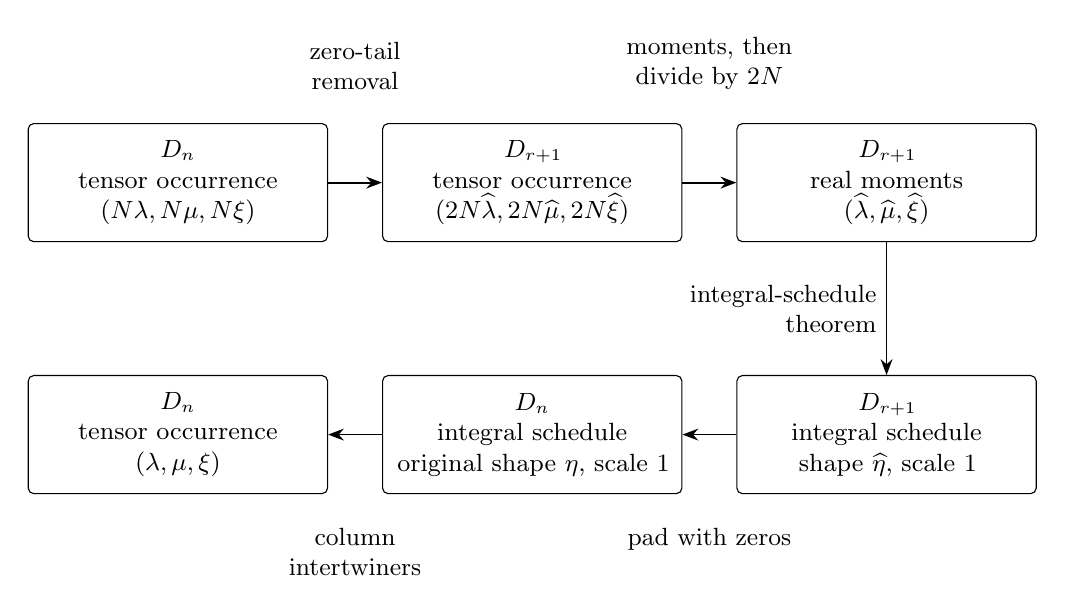
\begin{tikzpicture}[
  box/.style={draw,rounded corners=2pt,align=center,
    text width=3.45cm,minimum height=1.5cm,inner sep=5pt},
  arr/.style={-{Stealth[length=2mm]},line width=.65pt},
  every node/.style={font=\small}]
  \node[box] (original) at (0,0)
    {$D_n$\\tensor occurrence\\
     $(N\lambda,N\mu,N\xi)$};
  \node[box] (doubled) at (4.5,0)
    {$D_{r+1}$\\tensor occurrence\\
     $(2N\widehat\lambda,2N\widehat\mu,2N\widehat\xi)$};
  \node[box] (moment) at (9,0)
    {$D_{r+1}$\\real moments\\
     $(\widehat\lambda,\widehat\mu,\widehat\xi)$};
  \node[box] (smallpath) at (9,-3.2)
    {$D_{r+1}$\\integral schedule\\
     shape $\widehat\eta$, scale $1$};
  \node[box] (largepath) at (4.5,-3.2)
    {$D_n$\\integral schedule\\
     original shape $\eta$, scale $1$};
  \node[box] (conclusion) at (0,-3.2)
    {$D_n$\\tensor occurrence\\
     $(\lambda,\mu,\xi)$};
  \draw[arr] (original)--node[above=30pt,align=center]
    {zero-tail\\removal} (doubled);
  \draw[arr] (doubled)--node[above=30pt,align=center]
    {moments, then\\divide by $2N$} (moment);
  \draw[arr] (moment)--node[left,align=right]
    {integral-schedule\\theorem} (smallpath);
  \draw[arr] (smallpath)--node[below=30pt]
    {pad with zeros} (largepath);
  \draw[arr] (largepath)--node[below=30pt,align=center]
    {column\\intertwiners} (conclusion);
\end{tikzpicture}
\caption{The common-zero-tail branch, with $1\le r\le n-2$.
Here $\eta$ is a fundamental-column shape for the original
$D_n$ moving weight, and $\widehat\eta$ is its restriction to
the first $r+1$ coordinates. Doubling occurs only before passage
to real moments. Both integral schedules and the final tensor
occurrence use the original scale.}
\label{fig:zero-tail-scale}
\end{figure}


\begin{proof}[Proof of Theorem~\ref{thm:main}]
Suppose first that the invariant at scale \(N\in\Z_{>0}\) is nonzero.
Set \(\xi=\nu^*\), so \(V(N\xi)\) occurs in
\(V(N\lambda)\otimes V(N\mu)\), and
\(\lambda+\mu-\xi\) lies in the root lattice.
We may permute the three invariant labels before designating the
moving label \(\mu\).

If one of them has at most one zero coordinate, choose it as \(\mu\).
Lemma~\ref{lem:invariant-moment}, followed by division by \(N\),
gives a real moment solution for \(\lambda,\mu,\xi\).
Choose the shape \(\eta\) made of successive fundamental columns
summing to \(\mu\).
Theorem~\ref{thm:integral-schedule} gives an integral schedule for
this shape, and Proposition~\ref{prop:columns} gives
\(V(\lambda)\otimes V(\mu)\longrightarrow V(\xi)\) nontrivially.
This is the desired invariant.

Otherwise all three labels have at least two zero coordinates.
They are then integer-coordinate weights, nonnegative and supported
on initial coordinate segments.  Choose a label of largest support
as \(\mu\), and denote its support length by \(r\le n-2\).
If \(r=0\), all three representations are trivial.  Assume \(r\ge1\).
Apply Proposition~\ref{prop:zero-tail} to the occurrence at scale
\(N\).  It gives the occurrence in \(D_{r+1}\) for the truncated
labels at scale \(2N\).  Lemma~\ref{lem:invariant-moment}, divided
by \(2N\), therefore gives a real moment solution for the
\emph{unscaled} truncated labels.

Those labels remain integral, and their difference remains in
\(Q(D_{r+1})\): deleting zero coordinates preserves the even
coordinate sum.  The moving truncated label is positive in its first
\(r\) coordinates and has exactly one zero.  Take the fundamental
column shape for the original \(D_n\)-weight \(\mu\).
Since \(M_{r+1}=\cdots=M_n=0\), its fundamental expansion uses
only columns \(e_1+\cdots+e_k\) with \(k\le r\); every increment
therefore already vanishes beyond the retained coordinates.
Restrict each increment to the first \(r+1\) coordinates.
These increments are dominant for \(D_{r+1}\).  They need not be its
fundamental weights; Theorem~\ref{thm:integral-schedule} applies to
this arbitrary dominant-increment shape and gives an unscaled
integral schedule.

Pad this schedule with zero coordinates.  Its roots and even signed
permutations belong to \(D_n\), its endpoint lies in the required
full Weyl orbit, and every switch coefficient and sign is unchanged.
It is therefore an integral schedule for the \emph{original}
fundamental column shape.  Proposition~\ref{prop:columns} again
gives the unscaled invariant.  The use of \(2N\) supplied only real
existence in smaller rank and has introduced no saturation factor.

Conversely, let an unscaled invariant functional be nonzero.
The compact translates of highest-weight vectors span each
irreducible representation, so the functional is nonzero on some
triple of flag vectors.  Its \(N\)-th tensor power is nonzero on the
\(N\)-th powers of those same flag vectors.  Those powers lie in the
Cartan summands of highest weights \(N\lambda,N\mu,N\nu\).
Restriction gives the invariant at scale \(N\).

The arguments include \(D_2=A_1\times A_1\) and \(D_3=A_3\) with
the stated conventions.  If \(\Spin(2)\) is included, it is a torus;
its representations are characters, and the assertion is the
equivalence of the weight-sum equation with its positive integral
multiple.  This completes the proof.
\end{proof}

\begin{remark}[The stretching parameter]\label{tail:fractional}
Positive integral stretching is essential to the formulation.
If arbitrary positive rational \(N\) are allowed whenever all the
scaled weights exist, the unscaled root-lattice condition alone does
not suffice.  For \(D_n\), \(n\ge4\), take
\(\lambda=\mu=\nu=2e_1\).
The triangle contraction
\[
 (x,y)(y,z)(z,x)
\]
of the standard orthogonal form defines a nonzero invariant on
\(V(2e_1)^{\otimes3}\).
Indeed isotropic squares lie in the highest-weight module
\(V(2e_1)\), and, in a hyperbolic basis \(a_i,b_i\) with
\((a_i,b_j)=\delta_{ij}\), the isotropic vectors
\[
 a_1,\qquad b_1,\qquad a_1+b_1+a_2-b_2
\]
have nonzero pairwise products.  At \(N=1/2\) the three labels are
\(e_1\), whose sum \(3e_1\) is outside \(Q(D_n)\); hence the triple
has no invariant.  This does not affect
Theorem~\ref{thm:main}, where \(N\) is a positive integer.
\end{remark}

\bibliographystyle{plain}
\bibliography{references}
\end{document}
